\documentclass[12pt,a4paper]{article}

\usepackage[utf8]{inputenc}
\usepackage[T1]{fontenc}
\renewcommand{\figurename}{Figura}
\usepackage{amsmath,amssymb}
\usepackage{geometry}
\usepackage{xcolor}
\usepackage{float}
\usepackage{longtable,array,booktabs}
\usepackage{tikz}
\usetikzlibrary{arrows.meta,decorations.markings,calc}

\geometry{margin=2.5cm}
\setlength{\parskip}{0.35em}

% ------------------------------------------------------------
% Notacao das notas originais
% ------------------------------------------------------------
\newcommand{\Hb}{\overline{\mathcal{H}}}
\newcommand{\sh}{\widehat{\sigma}}
\newcommand{\Kh}{\widehat{K}}
\newcommand{\Jh}{\widehat{J}}
\newcommand{\Lh}{\widehat{L}}
\newcommand{\Gh}{\widehat{\Gamma}}
\newcommand{\sen}{\operatorname{sen}}

% ------------------------------------------------------------
% Marcacao das correcoes (tudo em vermelho)
%   \corr{..}        trecho corrigido (texto ou formula)
%   \nota{rot}{..}   nota numerada C1, C2, ... explicando a correcao
%   \ver{rot}        remissao a uma nota
% ------------------------------------------------------------
\newcommand{\corr}[1]{\textcolor{red}{#1}}
\newcommand{\cmais}{\mathbin{\textcolor{red}{+}}}
\newcommand{\cmenos}{\mathbin{\textcolor{red}{-}}}
\newcounter{corr}
\newcommand{\nota}[2]{\refstepcounter{corr}\label{#1}%
  {\color{red}\small[\textbf{C\thecorr}~---~#2]}}
\newcommand{\ver}[1]{{\color{red}\small[ver~C\ref{#1}]}}
\newcommand{\Cref}[1]{\textbf{C\ref{#1}}}

\tikzset{
  meio/.style={postaction={decorate},
    decoration={markings,mark=at position #1 with {\arrow{Stealth[length=2.2mm]}}}},
  meio/.default=0.55}

\begin{document}

\begin{center}
{\large\bfseries Tópicos de Física Estatística - IFUSP - 2026}\\[2pt]
{\large\bfseries Introdução à técnica de grupo de renormalização no espaço dos momentos}\\[8pt]
\fcolorbox{red}{white}{\parbox{0.92\textwidth}{\color{red}\small
\textbf{Versão anotada.} O texto em preto reproduz as notas originais
(revisão de 2/11/2026), com a mesma numeração de equações. Tudo o que está
em \textbf{vermelho} é correção ou comentário desta revisão: o trecho
corrigido aparece em vermelho no próprio lugar, seguido de uma nota numerada
[\textbf{C1}], [\textbf{C2}], \dots{} que diz o que estava no original e por
quê. A lista completa está no Apêndice~A; as contas refeitas para conferir
os pontos principais estão no Apêndice~B.}}
\end{center}

\bigskip

A função de partição de um modelo de Ising pode ser escrita na forma de
uma soma sobre configurações,
\begin{equation}
Z_I=\sum_{\{\sigma_r\}}\exp\left\{\frac12\sum_{r,r'}\beta J_{r,r'}\sigma_r\sigma_{r'}
+\sum_r\beta H\sigma_r\right\},
\end{equation}
em que $\sigma_r=\pm1$ é uma variável de spin no sítio $\vec r$ de uma rede cristalina,
a primeira soma é sobre as configurações dos spins, e as outras duas somas
são sobre os sítios da rede. A interação de troca,
$J_{r,r'}=J\left(|\vec r\,'-\vec r|\right)$, pode
ser bem geral, mas deve depender apenas da distância entre dois sítios da
rede; $H$ é o campo externo aplicado, $\beta$ é o inverso da temperatura e $J_{r,r'}>0$
no caso ferromagnético. Para simplificar a notação, desde que não haja
ambiguidades, vamos omitir os símbolos de vetor nas posições dos sítios da
rede.

Com o objetivo de contornar as dificuldades de uma soma discreta sobre
configurações, Mark Kac propôs em 1947 o ``modelo gaussiano'', versão
solúvel muito simplificada do modelo de Ising, com variáveis de spin
contínuas, assumindo valores entre $-\infty$ e $+\infty$, mas com um peso gaussiano
para assegurar a convergência das integrais (ver as reminiscências de Kac
em Physics Today \textbf{17}, \#10, 40, 1964). A função de partição desse ``modelo
gaussiano'' é dada por
\begin{equation}
Z_G=\prod_r\left[\int_{-\infty}^{+\infty}d\sigma_r\exp\left(-\frac12\sigma_r^2\right)\right]
\exp\left\{\frac12\sum_{r,r'}\beta J_{r,r'}\sigma_r\sigma_{r'}+\sum_r\beta H\sigma_r\right\}.
\end{equation}
A forma quadrática do integrando pode ser diagonalizada através de uma
transformação de Fourier. Esse problema é solúvel em qualquer dimensão,
mesmo na presença de campo externo, mas o comportamento crítico é do
tipo campo médio. Além disso, como ocorre uma ``catástrofe de baixas
temperaturas'', pois as integrais divergem abaixo de determinada temperatura
crítica, houve pouco interesse pelo modelo gaussiano durante certo tempo.
Mas esse modelo se tornou útil novamente quando se percebeu que o próprio
modelo de Ising tem um comportamento crítico do tipo campo médio acima
de $d=4$ dimensões. Tornou-se então interessante considerar uma versão do
modelo de Ising com variáveis de spin contínuas, mas não deixando de incluir
um termo de quarta ordem, que poderia ser tratado perturbativamente.
Apesar de algumas tentativas, as teorias de perturbação nunca deram conta do
comportamento crítico desse ``modelo quártico'' em três dimensões. Quando
surgiram as primeiras propostas de análise do comportamento crítico através
das idéias do grupo de \corr{renormalização}, esse tipo \corr{de} hamiltoniano, inspirado no
modelo gaussiano e na forma da energia livre de Landau-Ginzburg, mostrou-se
especialmente adequado para um tratamento perturbativo, com base no
parâmetro pequeno $\epsilon=4-d$, em torno da solução gaussiana em quatro
dimensões.
\nota{c:renorm}{digitação: no original, ``renormaliçao'' e ``esse tipo hamiltoniano''.}

Devemos também fazer referência a uma transformação integral, associada
a Hubbard e \corr{Stratonovich}, que permite uma representação contínua das
variáveis discretas do modelo de Ising.
\nota{c:strat}{grafia: no original, ``Stratonovitch''.}

Na primeira parte dessas notas definimos o modelo gaussiano, introduzimos
transformadas de Fourier na rede, e obtemos resultados exatos para
as funções termodinâmicas e para as formas assintóticas das correlações de
pares. Esperamos que essas notas sirvam como introdução elementar a
conceitos que permanecem muito úteis em física da matéria condensada e teoria
de campos.

Vale a pena mencionar que, devido às limitações do modelo gaussiano, o
próprio Mark Kac propôs um modelo alternativo, com variáveis de spin
contínuas, mas submetidas a um vínculo global ao invés dos vínculos gaussianos
individuais. A função de partição desse ``modelo esférico'' é dada por
\begin{equation}
Z_E=\prod_r\left[\int_{-\infty}^{+\infty}d\sigma_r\right]
\delta\left(\sum_r\sigma_r^2-N^d\right)
\exp\left\{\frac12\sum_{r,r'}\beta J_{r,r'}\sigma_r\sigma_{r'}+\sum_r\beta H\sigma_r\right\},
\end{equation}
em que o argumento da função delta de Dirac contém o ``vínculo esférico''
($N^d$ é o número total de sítios de uma rede $d$-dimensional). Introduzindo
uma representação integral da função delta e recorrendo à representação de
Fourier, é possível reduzir o problema a uma única integral que pode ser
obtida no limite termodinâmico (por uma aplicação judiciosa do método do
ponto de sela). Esse modelo esférico também é solúvel em qualquer dimensão,
mesmo na presença de campo externo, produzindo expoentes críticos que
diferem das previsões usuais de campo médio (mas que também diferem das
experiências). Apesar de um tanto distante da realidade física, o modelo
esférico tem sido utilizado como excelente laboratório para testes das teorias
sobre o comportamento crítico.

Nessas notas vamos mostrar que o modelo gaussiano é particularmente
adequado para um cálculo de grupo de renormalização no espaço dos momentos,
preservando graus de liberdade associados a pequenos momentos (grandes
comprimentos de onda). Introduzimos então o hamiltoniano de
Landau-Ginzburg-Wilson, cujo comportamento crítico deve pertencer à mesma classe
de universalidade do modelo de Ising. Desenvolvemos em seguida um cálculo
perturbativo, baseado na expansão de Wilson-Fisher em torno de $d=4$
dimensões, com o objetivo de obter o expoente crítico térmico do hamiltoniano
de Landau-Ginzburg-Wilson em primeira ordem em $\epsilon=4-d>0$.

Esse texto deve ser lido com boa dose de cautela, pois ainda pode haver
um certo número de pontos obscuros (e de errinhos)!

% ============================================================
\section{Modelo gaussiano}
% ============================================================

Utilizando a notação conhecida da física estatística, a função de partição do
modelo gaussiano pode ser escrita na forma
\begin{equation}
Z_G=\left[\prod_r\int_{-\infty}^{+\infty}d\sigma_r\right]\exp\left[\Hb_G\right],
\end{equation}
com o hamiltoniano efetivo
\begin{equation}
\Hb_G=\frac12\sum_{r,r'}\beta J_{r,r'}\sigma_r\sigma_{r'}+\sum_r\beta H_r\sigma_r-\sum_r\frac12\sigma_r^2,
\end{equation}
em que estamos aplicando um campo externo $H_r$ dependendo do sítio da
rede. As somas são sobre os sítios de uma rede hipercúbica $d$-dimensional
e o parâmetro de troca $J_{r,r'}=J\left(|r'-r|\right)$ depende apenas da distância de
separação entre os sítios $\vec r$ e $\vec r\,'$.

Adotando condições periódicas de contorno, introduzimos a transformada
discreta de Fourier,
\begin{equation}
\sigma_r=\frac{1}{N^{d/2}}\sum_q\sh_q\exp\left(iqr\right),
\end{equation}
em que o vetor $q$ pertence à ``primeira zona de Brillouin''.

Usando a condição de ortogonalidade,
\begin{equation}
\sum_r\exp\left[i\left(q+q'\right)r\right]=N^d\delta_{q,-q'},
\end{equation}
é fácil mostrar que
\begin{equation}
\begin{split}
\Hb_G&=\frac12\sum_{r,r'}\beta J_{r,r'}\sigma_r\sigma_{r'}+\sum_r\beta H_r\sigma_r-\sum_r\frac12\sigma_r^2=\\
&=\frac12\sum_q\left[\Kh(q)-1\right]\sh_q\sh_{-q}+\sum_q\sh_q\Lh_{-q},
\end{split}
\end{equation}
com as definições
\begin{equation}
\Kh(q)=\sum_h\beta J\left(|h|\right)\exp\left(-iqh\right)
\end{equation}
e
\begin{equation}
\Lh_q=\frac{1}{N^{d/2}}\sum_r\beta H_r\exp\left(-iqr\right)
\end{equation}

\begin{center}********************\end{center}

Vamos agora fazer algumas observações:

(i) Considerando (por simplicidade) um caso unidimensional, com parâmetro
de rede unitário, as condições periódicas de contorno implicam que
\begin{equation}
\exp\left(iqN\right)=1.
\end{equation}
Portanto, supondo que o número $N$ de sítios seja par, a primeira zona de
Brillouin é definida pela escolha
\begin{equation}
q=0,\pm\frac{2\pi}{N},\pm2\frac{2\pi}{N},...,\pm\left(\frac N2-1\right)\frac{2\pi}{N},\pi.
\end{equation}
Essa escolha, que deve ser conferida, não é necessária, mas é muito
conveniente. Note que existem sempre $N$ valores de $q$.

(ii) A variável de spin $\sigma_r$ é real. Levando em conta a escolha da zona de
Brillouin, temos então
\begin{equation}
\sum_q\sh_q\exp\left(iqr\right)=\sum_q\sh_q^{*}\exp\left(-iqr\right)=\sum_q\sh_{-q}^{*}\exp\left(iqr\right),
\end{equation}
ou seja,
\begin{equation}
\sh_q=\sh_{-q}^{*},
\end{equation}
indicando que a introdução de variáveis de spin complexas não altera o
número de graus de liberdade do sistema. É conveniente escrever $\sh_q$ em
termos das partes real e imaginária,
\begin{equation}
\sh_q=\frac{1}{\sqrt2}\left(R_q+iI_q\right),\qquad\forall q\neq0,
\end{equation}
de onde vem que
\begin{equation}
R_q=R_{-q}\,;\qquad I_q=-I_{-q}.
\end{equation}
Notem que $\sh_0=R_0$ é uma variável real.
\nota{c:qpi}{observação: a rigor, o ponto de borda $q=\pi$ da eq.~(12)
também satisfaz $q\equiv-q$ (módulo $2\pi$) e corresponde a uma variável real, como $q=0$.
Isso não altera a eq.~(20) nem qualquer resultado no limite termodinâmico.}

(iii) Usando essas definições, temos
\begin{equation}
\sum_r\sigma_r^2=\sum_q\sh_q\sh_{-q}=R_0^2+\sum_{q\neq0}\frac12\left(R_q^2+I_q^2\right),
\end{equation}
ou seja,
\begin{equation}
\sum_r\sigma_r^2=R_0^2+\sum_{q>0}\left(R_q^2+I_q^2\right),
\end{equation}
em que a soma é feita sobre a ``metade positiva'' da primeira zona de Brillouin.
A partir dessas considerações justificamos a transformação jacobiana
\begin{equation}
\left[\prod_r\int_{-\infty}^{+\infty}d\sigma_r\right](...)=
\int_{-\infty}^{+\infty}dR_0\left[\prod_{q>0}\int_{-\infty}^{+\infty}dR_q\int_{-\infty}^{+\infty}dI_q\right](...).
\end{equation}

\begin{center}*********************\end{center}

Na presença de um campo uniforme, $H_r=H$ para todo $r$, fica trivial
realizar as integrações gaussianas e escrever a função de partição do modelo
gaussiano,
\begin{equation}
Z_G=\exp\left\{\frac{N^dH^2\beta^2}{2\left[1-\Kh(0)\right]}\right\}
\prod_q\left[\frac{2\pi}{1-\Kh(q)}\right]^{1/2},
\end{equation}
em que a produtória é sobre todos os pontos da primeira zona de Brillouin. É
importante conferir com cuidado os termos dessa expressão. Note que $\Kh(q)$
é sempre real, e que $\Kh(q)=\Kh(-q)$.
\nota{c:paren}{digitação: no original há um parêntese a mais, ``$\Kh(q)=\Kh(-q))$''.}

Nesse ponto o problema está praticamente resolvido. A partir de $Z_G$
podemos obter o comportamento termodinâmico do sistema. No entanto,
essa forma de $Z_G$ indica que o modelo gaussiano não faz sentido para
\begin{equation}
1-\Kh(q)=1-\beta\Jh(q)<0,
\end{equation}
ou seja, para
\begin{equation}
k_BT<\max_q\Jh(q).
\end{equation}
Portanto, há uma temperatura limite, ou temperatura crítica $T_c$, dada por
\begin{equation}
k_BT_c=\max_q\Jh(q).
\end{equation}

% ------------------------------------------------------------
\subsection{Ferromagneto gaussiano numa rede hipercúbica}
% ------------------------------------------------------------

Restringindo o problema a um modelo ferromagnético com interações $J>0$
entre primeiros vizinhos numa rede hipercúbica em $d$ dimensões, com
parâmetro de rede unitário, temos
\begin{equation}
\Kh(q)=\sum_h\beta J\left(|h|\right)\exp\left(-iqh\right)=2\beta J\sum_{j=1}^d\cos q_j,
\end{equation}
ou seja,
\begin{equation}
\Kh(q)=2\beta Jd-\beta Jq^2+O\left(q^4\right),
\end{equation}
que assume um valor máximo, $\Kh(0)=2\beta Jd$, para $q=0$.

A magnetização por spin é dada por
\begin{equation}
m=\frac{1}{\beta N^d}\frac{\partial}{\partial H}\ln Z_G=\frac{\beta H}{1-\Kh(0)},
\end{equation}
que se anula para $H=0$ (e não existe abaixo de $T_c$). Acima da temperatura
crítica, temos a suscetibilidade magnética,
\begin{equation}
\chi=\frac{\partial m}{\partial H}=\frac{\beta}{1-\Kh(0)}=\frac{\beta}{1-2\beta Jd}=\frac{1}{k_BT-2Jd},
\end{equation}
que diverge, com expoente $\gamma=1$, na temperatura crítica $T_c=2Jd/k_B$.

Nas vizinhanças do ponto crítico, a magnetização contra o campo pode
ser representada por uma curva universal (desde que sejam feitos gráficos de
$m/t^{\beta}$ contra $H/t^{\beta+\gamma}$, em que $t=\left(T-T_c\right)/T_c$ e os expoentes $\beta$ e $\gamma$ assumem
os valores usuais de campo médio).
\nota{c:scal}{observação: no modelo gaussiano $m=H/(k_BT_c\,t)$ é linear em $H$ e
não há magnetização espontânea, de modo que o colapso vale para qualquer $\beta$
e só ficam definidos $\gamma=1$ e a combinação $\Delta=\beta+\gamma$. Pela eq.~(77),
$\Delta=1/2+d/4$, que coincide com o valor de campo médio, $3/2$, apenas em $d=4$.}

A campo nulo, a energia interna por spin é dada por
\begin{equation}
u=-\frac{1}{2N^d}\sum_q\frac{\Jh(q)}{1-\Kh(q)}.
\end{equation}
No limite termodinâmico, temos
\begin{equation}
u=-\frac{1}{2\left(2\pi\right)^d}\int d^dq\,\frac{\Jh(q)}{1-\Kh(q)}.
\end{equation}
Notem que aparecem estruturas semelhantes na solução do modelo de Ising na
rede quadrada. Essa integral deve ser feita na zona de Brillouin, certamente
havendo problemas nas vizinhanças de $q=0$. Por exemplo, na temperatura
crítica devemos analisar o comportamento em $q=0$ da integral
\begin{equation}
\int_0q^{d-1}dq\,\frac{1}{q^2}=\frac{1}{d-2}\left.q^{d-2}\right|_0,
\end{equation}
que diverge para $d\corr{\,\leq\,}2$ (pois não teria sentido uma energia interna infinita!).
\nota{c:d2}{no original, ``$d<2$''. Em $d=2$ o integrando é $dq/q$ e a integral
também diverge (logaritmicamente); a primitiva em (30) vale só para $d\neq2$.}

O calor específico a campo nulo é dado por
\begin{equation}
c_{H=0}=\frac12k_B\frac{1}{N^d}\sum_q\left[\frac{\Kh(q)}{1-\Kh(q)}\right]^2.
\end{equation}
Para analisar o comportamento crítico, transformamos a soma numa integral
e retemos apenas os termos dominantes, para $q$ pequeno, no numerador e no
denominador. Temos então a forma assintótica
\begin{equation}
c_{H=0}\sim\frac12k_B\frac{1}{N^d}\frac{N^d}{\left(2\pi\right)^d}\int C_dq^{d-1}dq\,
\frac{\left(2\beta Jd\right)^2}{\left[\Delta T+\beta Jq^2\right]^{\corr{2}}},
\end{equation}
\noindent\nota{c:c32}{erro de conta: no original falta o expoente 2 no denominador.
Ele vem do quadrado em (31) e é indispensável para obter (34):
$\int q^{d-1}dq/(\Delta T+\beta Jq^2)^2\sim t^{d/2-2}$, enquanto sem o quadrado
resultaria $t^{d/2-1}$.}

\noindent em que
\begin{equation}
\Delta T=1-2\beta Jd
\end{equation}
vai a zero no ponto crítico, e a constante $C_d$ incorpora o resultado de
integrações angulares. Fazendo uma pequena manipulação algébrica, ainda é
fácil mostrar que
\begin{equation}
c_{H=0}\sim t^{\frac d2-2},
\end{equation}
ou seja, o calor específico a campo nulo comporta-se com o expoente
$\alpha=2-d/2$ (com $\alpha=0$ quando $d=4$). O calor específico certamente não diverge
para $d\corr{\,>\,}4$\corr{; em $d=4$ há uma divergência logarítmica,
$c_{H=0}\sim-\ln t$}.
\nota{c:d4log}{no original, ``não diverge para $d\geq4$''. Em $d=4$,
$\int_0^1q^3dq/(t+q^2)^2=-\tfrac12\ln t+O(1)$: o expoente $\alpha=0$ corresponde a
uma divergência logarítmica, não a um valor finito.}

% ------------------------------------------------------------
\subsection{Correlações gaussianas}
% ------------------------------------------------------------

As correlações de dois pontos (spin-spin) são dadas por
\begin{equation}
\Gamma\left(r,r'\right)=\left\langle\sigma_r\sigma_{r'}\right\rangle=
\frac{1}{N^d}\sum_{q\corr{,q'}}\exp\left[iq\cdot r+iq'\cdot r'\right]\left\langle\sh_q\sh_{q'}\right\rangle,
\end{equation}
em que, por simplicidade, não estamos utilizando a notação vetorial.
\nota{c:sum35}{notação: no original a soma é só sobre $q$, mas o somando depende de
$q$ e de $q'$; a soma é dupla, e se reduz à soma simples de (42) por causa de (41).}

Levando em conta a representação das variáveis complexas de spin em
termos das componentes reais e imaginárias, dada pela eq. (15), temos
\begin{equation}
\left\langle\sh_q\sh_{q'}\right\rangle=\frac12\left\langle R_qR_{q'}+iR_qI_{q'}+iI_qR_{q'}-I_qI_{q'}\right\rangle.
\end{equation}
Como não há acoplamentos entre as variáveis $R_q$ e $I_q$, temos uma expressão
mais simples,
\begin{equation}
\left\langle\sh_q\sh_{q'}\right\rangle=\frac12\left\langle R_qR_{q'}\right\rangle-\frac12\left\langle I_qI_{q'}\right\rangle.
\end{equation}
Também é fácil verificar que
\begin{equation}
\left\langle\sh_q\sh_q\right\rangle=\frac12\left\langle R_qR_q\right\rangle-\frac12\left\langle I_qI_q\right\rangle=0,
\end{equation}
\begin{equation}
\left\langle\sh_q\sh_{-q}\right\rangle=\frac12\left\langle R_qR_{-q}\right\rangle-\frac12\left\langle I_qI_{-q}\right\rangle
=\frac12\left\langle R_q^2\right\rangle+\frac12\left\langle I_q^2\right\rangle=\left\langle R_q^2\right\rangle
\end{equation}
e
\begin{equation}
\left\langle\sh_q\sh_{q'}\right\rangle=0\quad\text{para}\quad q'\neq-q.
\end{equation}
Resumindo, podemos escrever
\begin{equation}
\left\langle\sh_q\sh_{q'}\right\rangle=\left\langle\sh_q\sh_{-q}\right\rangle\delta_{q',-q}
\end{equation}
e
\begin{equation}
\left\langle\sigma_r\sigma_{r'}\right\rangle=\frac{1}{N^d}\sum_q\exp\left[iq\cdot(r-r'\corr{)}\right]\left\langle\sh_q\sh_{-q}\right\rangle,
\end{equation}
ficando bem evidente a simetria translacional.
\nota{c:par42}{digitação: no original falta fechar o parêntese, ``$\exp[iq\cdot(r-r']$''.}
Resta agora notar que
\begin{equation}
\Gh(q)=\left\langle\sh_q\sh_{-q}\right\rangle=\left\langle R_q^2\right\rangle=\frac{1}{1-\Kh(q)},
\end{equation}
que é a expressão conhecida do ``propagador gaussiano''. Verificar \corr{com} cuidado
esse cálculo!
\nota{c:cm}{digitação: no original, ``cm cuidado''.}

Finalmente podemos escrever as correlações de dois pontos,
\begin{equation}
\Gamma(r)=\Gamma(r,0)=\frac{1}{N^d}\sum_q\exp\left(iq\cdot r\right)\frac{1}{1-\Kh(q)}.
\end{equation}
No limite termodinâmico, para um ferromagneto numa rede hipercúbica
simples, com interações de primeiros vizinhos, temos
\begin{equation}
\Gamma(r)=\frac{1}{\left(2\pi\right)^d}\int d^dq\,\frac{\exp\left(iq\cdot r\right)}{1-2\beta J\left(\cos q_1+\cos q_2+...+\cos q_d\right)},
\end{equation}
que é conhecida como uma ``função de Green na rede'' (e que lembra
expressões obtidas no contexto das soluções exatas para o modelo de Ising).

Nas vizinhanças da criticalidade, com $\Delta T=1-2\beta Jd\sim0$, a equação
(45) assume uma forma bem mais simples, restrita aos termos de pequenos
momentos (grandes comprimentos de onda) no denominador do integrando.
Então escrevemos a forma assintótica
\begin{equation}
\Gamma(r)=\frac{1}{\left(2\pi\right)^d}\int d^dq\,\frac{\exp\left(iq\cdot r\right)}{\Delta T+\beta Jq^2+...},
\end{equation}
que ainda pode ser simplificada se a zona de Brillouin for transformada num
objeto com simetria esférica, e a variável radial for tomada de 0 a $\infty$. Note
que o elemento de volume em $d$ dimensões é dado por
\begin{equation}
d^dq=q^{d-1}\sen^{d-2}\theta_1\sen^{d-3}\theta_2....\sen\theta_{d-2}\,d\corr{q}\,d\theta_1d\theta_2...d\theta_{d-1},
\end{equation}
\noindent\nota{c:dq47}{notação: no original, ``$dr$'' no lugar de ``$dq$'' (a variável radial aqui é $q$).}

\noindent e os limites de integração vão de 0 a $\pi$ para \corr{$\theta_1,\theta_2,...,\theta_{d-2}$}
e de 0 a $2\pi$ para \corr{$\theta_{d-1}$}. Para
$d\geq4$, não há o menor problema com essas integrais.
\nota{c:ang47}{no original, ``de 0 a $\pi$ para $\theta_1$ e de 0 a $2\pi$ para $\theta_2$, $\theta_3$, ...''.
Em coordenadas hiperesféricas só o último ângulo, $\theta_{d-1}$ (o que não aparece nos senos de (47)),
varia de 0 a $2\pi$; todos os outros variam de 0 a $\pi$.}

Pelo menos em três dimensões, $d=3$, nas vizinhanças da criticalidade
(isto é, com $\Delta T$ pequeno, mas $\Delta T\neq0$), é fácil obter um resultado analítico.
Nesse caso, descartando termos de ordem $q^4$ no denominador, temos a forma
assintótica
\begin{equation}
\begin{split}
\Gamma(r)&\sim\frac{1}{\left(2\pi\right)^3}2\pi\int_0^{\pi}\sen\theta\,d\theta\int_0^{\pi}q^2dq\,\frac{\exp\left(iqr\cos\theta\right)}{\Delta T+\beta Jq^2}=\\
&=\frac{1}{2\pi^2}\int_0^{\pi}q^2\left(\frac{\sen qr}{qr}\right)\frac{1}{\Delta T+\beta Jq^2}\,dq.
\end{split}
\end{equation}
Para obter a forma assintótica (com $\Delta T\to0$) que estamos procurando,
podemos estender os limites de integração. Então temos
\begin{equation}
\Gamma(r)\sim\int_{-\infty}^{+\infty}q^2\frac{\sen\left(qr\right)}{qr}\frac{1}{t+q^2}\,dq,
\end{equation}
que é uma integral dominada \corr{pelos} polos complexos, $q=\pm i\sqrt t$. Recorrendo
às técnicas usuais de integração complexa, obtemos finalmente a forma
assintótica (para $t\to0$ e $r\to\infty$)
\nota{c:polos}{digitação: no original, ``pelo polos''.}
\begin{equation}
\Gamma(r)\sim\frac1r\exp\left[-\frac r\xi\right],
\end{equation}
em que
\begin{equation}
\xi\sim t^{-1/2}
\end{equation}
é o comprimento de correlação, com o expoente crítico $\nu=1/2$. Ainda em
três dimensões, exatamente na temperatura crítica, isto é, fazendo $\Delta T=0$,
temos
\begin{equation}
\Gamma(r)\sim\frac{1}{\left(2\pi\right)^2}\frac{1}{\beta J}\int_0^{\pi}dq\int\limits_{-1}^{1}dx\exp\left(iqrx\right)\sim\frac1r,
\end{equation}
de onde vem o expoente $\eta=0$ associado ao decaimento das correlações
críticas.

Não é difícil mostrar, pelo menos qualitativamente, que esses resultados
ainda permanecem válidos para $d\geq4$, com a forma
\begin{equation}
\Gamma(r)\sim\frac{1}{r^{d-2}}\exp\left[-\frac r\xi\right]
\end{equation}
em que $\xi\sim t^{-1/2}$ é o resultado famoso de campo médio obtido pioneiramente
por Ornstein e Zernike.
\nota{c:oz53}{observação: (53) é exata só em $d=3$. Em $d$ dimensões a forma completa
é a da eq.~(57) corrigida, $\Gamma\sim r^{-(d-2)}(r/\xi)^{(d-3)/2}e^{-r/\xi}$ para $r\gg\xi$,
que se reduz a $r^{-(d-2)}$ para $\xi\to\infty$. Os expoentes $\nu=1/2$ e $\eta=0$ não mudam.}

O modelo gaussiano confirma então a nossa ideia sobre as correlações
críticas. Fora da criticalidade, as correlações decaem exponencialmente, com
um comprimento característico de decaimento, que se torna cada vez maior
ao nos aproximarmos do ponto crítico. Na criticalidade, não há comprimento
característico, pois as correlações decaem com uma lei de potência.

Vale a pena mencionar que há um artifício atribuído a Elliott Montroll
na consideração de funções de Green na rede, que pode ser utilizado para
obter resultados assintóticos em $d$ dimensões. A ideia consiste em considerar
a integral
\begin{equation}
I=\int\limits_{-\infty}^{+\infty}...\int\limits_{-\infty}^{+\infty}dq_1...dq_d\,\frac{\exp\left(i\vec q\cdot\vec r\right)}{q^2+\kappa^2}
\end{equation}
e utilizar a identidade
\begin{equation}
\int\limits_0^{\infty}\exp\left(-\tau x\right)dx=\frac1\tau
\end{equation}
para se livrar do denominador. Após manipulações elementares, temos a
integral
\begin{equation}
I=\int\limits_0^{\infty}dt\left(\frac\pi t\right)^{d/2}\exp\left(-\kappa^2t-\frac{r^2}{4t}\right),
\end{equation}
que pode ser expressa em termos de uma função de Bessel (ver a tabela de
Gradshteyn e Ryzhik, Academic Press, edições a partir de 1965). Para $\kappa=0$,
é fácil obter um decaimento da forma $I\sim1/r^{d-2}$, confirmando o expoente
$\eta=0$. Para $\kappa\neq0$, mas $\kappa\to0$, temos o resultado assintótico
\begin{equation}
I\sim\corr{\frac{1}{r^{d-2}}}\left(\kappa r\right)^{(d-3)/2}\exp\left(-\kappa r\right),
\end{equation}
confirmando o valor de campo médio, $\nu=\corr{1/2}$.

\noindent\nota{c:i57}{erro de conta: no original, $I\sim(\kappa r)^{(d-3)/2}\exp(-\kappa r)$, sem o
fator $1/r^{d-2}$. A integral (56) vale exatamente
$I=2\pi^{d/2}\left(2\kappa/r\right)^{\frac d2-1}K_{\frac d2-1}(\kappa r)$, e
$K_\mu(x)\simeq\sqrt{\pi/2x}\,e^{-x}$ para $x\gg1$ dá
$I\propto\kappa^{(d-3)/2}r^{-(d-1)/2}e^{-\kappa r}=r^{-(d-2)}(\kappa r)^{(d-3)/2}e^{-\kappa r}$.
A forma original cresce com $r$ no prefator para $d>3$ e, em $d=3$, daria $e^{-\kappa r}$
em vez do $e^{-\kappa r}/r$ da eq.~(50). Conferido numericamente (Apêndice~B).}

\noindent\nota{c:nu57}{erro: no original, ``$\nu=1$''. Como $\kappa=1/\xi\sim t^{1/2}$, o valor
de campo médio é $\nu=1/2$, como nas eqs.~(51) e (53).}

% ------------------------------------------------------------
\subsection{Renormalização do modelo gaussiano}
% ------------------------------------------------------------

A idéia do cálculo de grupo de renormalização no espaço dos momentos
consiste em integrar sobre as variáveis de spin associadas a valores grandes
do vetor de onda $q$, fazendo uma operação que é equivalente à eliminação
no espaço real dos graus de liberdade de curto alcance, dentro de bloquinhos
de dimensão $b>1$. Como os \corr{pequenos} comprimentos de onda (ou seja,
curtas distâncias) não devem influenciar o comportamento crítico, o primeiro
passo consiste em deformar a zona de Brillouin, que vai ser substituída por
uma esfera de raio unitário. Em seguida essa esfera é dividida num caroço
interno, de raio $1/b$, e numa coroa externa, com $1/b<q<1$ (ver a figura
1). A integração é feita apenas sobre os graus de liberdade correspondentes
a valores de $q$ na coroa externa.
\nota{c:lambda}{erro conceitual: no original, ``grandes comprimentos de onda (ou seja,
curtas distâncias)''. Curtas distâncias correspondem a $q$ grande, isto é, a \emph{pequenos}
comprimentos de onda; os grandes comprimentos de onda são justamente os que controlam o
comportamento crítico, como dito na introdução.}

Usando uma notação mais compacta, a função de partição do modelo
gaussiano pode ser escrita como
\begin{equation}
Z_G=\int\left[d\sh_q\right]\exp\left(\Hb_G\right),
\end{equation}
em que
\begin{equation}
\int\left[d\sh_q\right](...)=\int_{-\infty}^{+\infty}dR_0\left[\prod_{q>0}\int_{-\infty}^{+\infty}dR_q\int_{-\infty}^{+\infty}dI_q\right](...)
\end{equation}
e
\begin{equation}
\Hb_G=\frac12\sum_q\left[2\beta Jd-1-\beta Jq^2+O\left(q^4\right)\right]\sh_q\sh_{-q}+\beta HN^{d/2}R_0,
\end{equation}
em que estamos restringindo a análise a um modelo numa rede hipercúbica
de dimensão $d$, com interações ferromagnéticas entre primeiros vizinhos, na
presença de um campo externo uniforme. Como essa integral se fatoriza,
ainda podemos escrever
\begin{equation}
Z_G=\int^{<}\left[d\sh_q\right]\int^{>}\left[d\sh_q\right]\exp\left(\Hb_0^{<}+\Hb_0^{>}\right),
\end{equation}
em que os símbolos $<$ ou $>$ referem-se a valores de $q$ no caroço interno
(dentro) ou na coroa externa (fora) da zona de Brillouin.
\nota{c:h0}{observação: a partir daqui o hamiltoniano gaussiano passa a ser chamado
$\Hb_0$; isto é, $\Hb_0\equiv\Hb_G$ e $\Hb_G=\Hb_0^<+\Hb_0^>$.}
A integração sobre
os graus de liberdade correspondentes a valores de $q$ na coroa externa produz
uma função da temperatura bem comportada, pois as singularidades somente
se manifestam nas vizinhanças de $q=0$. Então temos
\begin{equation}
Z_G=f_0\left(T\right)\int^{<}\left[d\sh_q\right]\exp\left(\Hb_0^{<}\right),
\end{equation}

\begin{figure}[H]
\centering
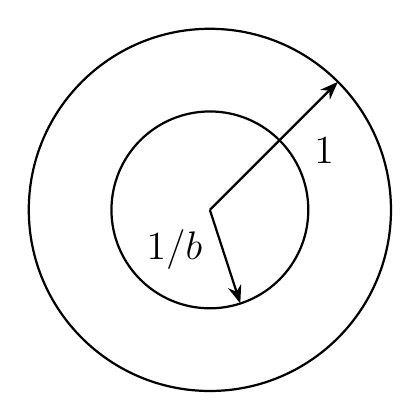
\begin{tikzpicture}[>=Stealth]
  \draw[thick] (0,0) circle (2.3);
  \draw[thick] (0,0) circle (1.25);
  \draw[->,thick] (0,0) -- (45:2.3);
  \draw[->,thick] (0,0) -- (-72:1.25);
  \node at (1.45,0.75) {\Large 1};
  \node at (-0.45,-0.5) {\Large $1/b$};
\end{tikzpicture}
\caption{Zona de Brillouin ($q<1$), dividida em um caroço interno ($q<1/b$)
e uma coroa externa ($1/b<q<1$).}
\end{figure}

\noindent com o hamiltoniano transformado
\begin{equation}
\Hb'=\Hb_0^{<}=\frac12\sum_{|q|<1/b}\left[2\beta Jd-1-\beta Jq^2+O\left(q^4\right)\right]\sh_q\sh_{-q}+\beta HN^{d/2}R_0.
\end{equation}

Vamos tornar essa expressão um pouco mais interessante introduzindo a
mudança de variáveis
\begin{equation}
\sh_q\to\frac{1}{\left(\beta J\right)^{1/2}}\sh_q
\end{equation}
e a notação
\begin{equation}
r=\frac{\corr{1-2\beta Jd}}{\beta J}\corr{{}=\frac{\Delta T}{\beta J}}.
\end{equation}
Como é comum na área, estamos usando $r$ ao invés de $t$; o ponto crítico deve
corresponder a $r=0$ (por favor, não confundam $r$ com a posição!). Temos
então
\begin{equation}
\Hb'=\corr{-}\frac12\sum_{|q|<1/b}\left[r\cmais q^2\cmenos\omega q^4+O\left(q^6\right)\right]\sh_q\sh_{-q}
+\frac{\beta HN^{d/2}}{\left(\beta J\right)^{1/2}}R_0,
\end{equation}

\noindent\fcolorbox{red}{white}{\parbox{0.97\textwidth}{\color{red}\small
\refstepcounter{corr}\label{c:rconv}%
[\textbf{C\thecorr}~---~\textbf{sinal de $r$: é a inconsistência mais importante destas notas.}
No original, a eq.~(65) é $r=(2\beta Jd-1)/(\beta J)$ e as eqs.~(66), (67), (70), (71),
(90), (91), (94), (105) e (125) trazem $\tfrac12[\,r-q^2\,]$. Com essa definição, $r<0$ acima de
$T_c$ e o propagador gaussiano, pelas eqs.~(43) e (25), é
$\langle\sh_q\sh_{-q}\rangle=1/(q^2-r)$. Mas as eqs.~(100)--(102), (119)--(122) e (130)--(133)
usam $1/(r+q^2)$, e as recorrências (106), (111) e (126) têm $+\tfrac12Ab^2u$: tudo isso só é
coerente com $r=(1-2\beta Jd)/(\beta J)=\Delta T/(\beta J)$, positivo acima de $T_c$ --- que é,
aliás, o que ``usar $r$ ao invés de $t$'' sugere.

\textbf{Correção adotada aqui:} trocar a definição de $r$ nas eqs.~(65) e (89) e, em
consequência, escrever $-\tfrac12[\,r+q^2\,]$ nas nove equações citadas. É a menor alteração que
deixa corretos, \emph{sem mais mudanças}, todos os resultados seguintes: $A$, $B$, as recorrências
(106), (111)--(112), (126)--(127), $u^*$, $r^*<0$, a figura~4 e $\lambda_1=2-\epsilon/3$.

\textbf{Alternativa equivalente:} manter $r=(2\beta Jd-1)/(\beta J)$ e trocar $r\to-r$ da
eq.~(100) em diante: propagador $1/(q^2-r)$, $r'=b^2r-\tfrac12Ab^2u$,
$\partial A/\partial r=+B$ e $r^*>0$ (com o ponto fixo de Ising acima do eixo $u$ na figura~4).

\textbf{Cuidado:} trocar \emph{apenas} o sinal da recorrência, $r'=b^2r-\tfrac12Ab^2u$, mantendo
$A=\int(r+q^2)^{-1}$, dá $\lambda_1=2+\epsilon/3$ e $\nu=\tfrac12-\tfrac{\epsilon}{12}$, que está
errado. No original os dois deslizes de sinal --- no propagador (100) e na recorrência (106) --- se
compensam, e por isso o resultado final (141)--(143) está correto. Ver o Apêndice~B.]}}

\medskip

\noindent em que foi explicitamente incluído um termo de ordem $q^4$ (e a soma se realiza
apenas sobre o ``caroço'' da zona de Brillouin). Transformando a soma numa
integral, temos
\begin{equation}
\Hb'=\corr{-}\frac12\frac{N^d}{\left(2\pi\right)^d}\int_0^{1/b}d^dq\left[r\cmais q^2\cmenos\omega q^4+O\left(q^6\right)\right]\sh_q\sh_{-q}
+\frac{\beta HN^{d/2}}{\left(\beta J\right)^{1/2}}R_0.
\end{equation}
\ver{c:rconv}

Para comparar com o hamiltoniano original, vamos restaurar os
comprimentos e a magnitude das variáveis de spin através das transformações de
escala
\begin{equation}
q'=bq\quad\to\quad q=\frac1bq'
\end{equation}
e
\begin{equation}
\sh_{\frac1bq'}\to b\,\sh'_{q'}.
\end{equation}
Essa última escolha, em particular, que mantém inalterado o coeficiente do
termo em $q^2$ do hamiltoniano, vai preservar o decaimento das correlações
críticas (isto é, o expoente crítico $\eta$). Num cálculo perturbativo de ordem
mais baixa, como no esquema de Wilson-Fisher que vamos utilizar mais
adiante, essa escolha ainda é suficiente.

Temos então o hamiltoniano transformado $\Hb'$, com $\left(N'\right)^d=\left(N/b\right)^d$ graus
de liberdade, que deve ser comparado com o hamiltoniano inicial,
\begin{equation}
\begin{split}
\Hb'=\corr{-}\frac12\frac{\left(N'\right)^d}{\left(2\pi\right)^d}\int_0^1d^dq'&\left[b^2r\cmais q'^2\cmenos\omega b^{-2}q'^4+O\left(q'^6\right)\right]\sh'_{q'}\sh'_{-q'}+\\
&+b^{1+\frac d2}\frac{\beta H\left(N'\right)^{d/2}}{\left(\beta J\right)^{1/2}}R'_0,
\end{split}
\end{equation}
ou seja,
\begin{equation}
\Hb'=\corr{-}\frac12\sum_{q'}\left[b^2r\cmais q'^2\cmenos\omega b^{-2}q'^4+O\left(q'^6\right)\right]\sh'_{q'}\sh'_{-q'}
+b^{1+\frac d2}\frac{\beta H\left(N'\right)^{d/2}}{\left(\beta J\right)^{1/2}}R'_0,
\end{equation}
\ver{c:rconv}
em que a soma é feita sobre uma zona de Brillouin com $\left(N'\right)^d=\left(N/b\right)^d$
pontos. Comparando com o hamiltoniano inicial, obtemos as relações de
recorrência
\begin{equation}
r'=b^2r,
\end{equation}
\begin{equation}
\omega'=b^{-2}\omega
\end{equation}
e
\begin{equation}
H'=b^{1+\frac d2}H.
\end{equation}
de onde vem o ponto fixo gaussiano (de natureza trivial),
\begin{equation}
r^*=\omega^*=H^*=0.
\end{equation}
O termo em $q^4$ é irrelevante (como também seriam os termos de ordem
superior). Os expoentes térmico e magnético são dados por
\begin{equation}
\lambda_1=2\qquad\text{e}\qquad\lambda_2=1+\frac d2,
\end{equation}
de onde obtemos
\begin{equation}
\alpha=2-\frac d2\qquad\text{e}\qquad\Delta=\beta+\gamma=\frac{\lambda_2}{\lambda_1}=\frac12+\frac d4.
\end{equation}
Para $d=4$, recuperamos os valores usuais de campo médio.

% ============================================================
\section{Modelo de Landau-Ginzburg-Wilson}
% ============================================================

A presença de um termo de quarta ordem na expressão da energia livre
de Landau é essencial para descrever o comportamento nas vizinhanças do
ponto crítico de um ferromagneto simples. De acordo com a teoria de
Landau, adotando a linguagem do ferromagnetismo uniaxial, escrevemos uma
densidade de energia livre,
\[
f\left[m(r)\right]=A\left[m(r)\right]^2+B\left[\nabla m(r)\right]^2+C\left[m(r)\right]^4,
\]
em que o termo de gradiente leva em conta a variação espacial, mas não
quebra a simetria do sistema. Além disso, devemos ter $A=A_0\left(T-T_C\right)$; as
constantes $A_0$, $B$ e $C$ devem ser positivas. A energia livre $F$ do sistema é
uma integral no espaço real,
\begin{equation}
F=\int d^3r\,f\left[m(r)\right]=\int d^3r\left\{A\left[m(r)\right]^2+B\left[\nabla m(r)\right]^2+C\left[m(r)\right]^4\right\}.
\end{equation}

Essa energia livre de Landau pode ser vista como um ``hamiltoniano de
grão grosso'' do sistema, em que já se eliminaram graus de liberdade atuando
a curtíssimas distâncias. Podemos então utilizar a notação de integrais
funcionais para escrever a função canônica de partição
\begin{equation}
Z=\int\left[dm(r)\right]\exp\left\{-\beta\int d^3r\,f\left[m(r)\right]\right\},
\end{equation}
que é semelhante à expressão para o modelo gaussiano, mas com a adição
de um termo extra de ordem quártica, que torna intransponível qualquer
cálculo exato (a aproximação de campo médio seria uma mera ``solução de
ponto de sela'' dessa integral). Levando em conta a universalidade do
comportamento crítico, esse hamiltoniano de grão grosso, que ficou conhecido
como ``hamiltoniano de Ginzburg-Landau-Wilson'', deve ter o mesmo
comportamento crítico do modelo de Ising.

Vamos então considerar o modelo gaussiano, com a adição de um termo
quártico,
\begin{equation}
\Hb=\Hb_G+\Hb_p,
\end{equation}
em que $\Hb_G$ é o hamiltoniano usual do modelo gaussiano (ferromagnético,
numa rede cúbica $d$-dimensional, com interações de primeiros vizinhos) e o
termo perturbativo é dado por
\begin{equation}
\Hb_p=-\widetilde u\sum_r\sigma_r^4=-\frac{\widetilde u}{N^d}\sum_{q_1,q_2,q_3,q_4}\sh_{q_1}\sh_{q_2}\sh_{q_3}\sh_{q_4}\delta_{q_1+q_2+q_3+q_4,0}\,,
\end{equation}
em que $\widetilde u>0$ é um parâmetro positivo. Devido a esse termo quártico,
aparecem acoplamentos ``dentro'' e ``fora'' da esfera de raio $1/b$. Mantendo a
mesma notação do caso gaussiano, temos
\begin{equation}
\Hb=\Hb_0^{<}+\Hb_0^{>}+\Hb_p.
\end{equation}
A função de partição é dada por
\begin{equation}
\begin{split}
Z&=\int^{<}\left[d\sh_q\right]\int^{>}\left[d\sh_q\right]\exp\left[\Hb_0^{<}+\Hb_0^{>}+\Hb_p\right]=\\
&=\int^{<}\left[d\sh_q\right]\exp\left[\Hb_0^{<}\right]\int^{>}\left[d\sh_q\right]\exp\left[\Hb_0^{>}+\Hb_p\right].
\end{split}
\end{equation}
Definindo um valor esperado em relação a $\Hb_0^{>}$,
\begin{equation}
\left\langle\exp\left[\Hb_p\right]\right\rangle_{0>}=\frac{1}{Z_{0>}}\int^{>}\left[d\sh_q\right]\exp\left[\Hb_0^{>}+\Hb_p\right],
\end{equation}
em que $Z_{0>}$ é uma função bem comportada da temperatura,
\begin{equation}
Z_{0>}=\int^{>}\left[d\sh_q\right]\exp\left[\Hb_0^{>}\right],
\end{equation}
temos
\begin{equation}
Z=Z_{0>}\int^{<}\left[d\sh_q\right]\exp\left[\Hb_0^{<}\right]\left\langle\exp\left[\Hb_p\right]\right\rangle_{0>},
\end{equation}
que está na forma adequada para um tratamento perturbativo.

\textbf{A idéia do esquema de grupo de renormalização de Wilson-Fisher consiste em:}

\textbf{(i) fazer uma expansão perturbativa em torno da dimensão $d=4$;}

\textbf{(ii) escolher um parâmetro pequeno, $\epsilon=4-d$;}

\textbf{(iii) supor que $\widetilde u$ seja de ordem $\epsilon$, e que o expoente $\eta$ associado
ao decaimento das correlações críticas seja de ordem $\epsilon^2$.}

O tratamento perturbativo até segunda ordem se baseia na expansão de
cumulantes
\begin{equation}
\left\langle\exp\left[\Hb_p\right]\right\rangle=\exp\left\{\left\langle\Hb_p\right\rangle+\frac12\left[\left\langle\Hb_p^2\right\rangle-\left\langle\Hb_p\right\rangle^2\right]+...\right\},
\end{equation}
em que a forma do termo quadrático, com um sinal menos intermediário, é
providencial (na linguagem dos grafos, isso significa que podem ser
descartados os grafos desconexos). Vamos fazer os cálculos e verificar a posteriori a
consistência dessas hipóteses.

Preparando um pouco mais o hamiltoniano, é conveniente fazer a
transformação de variáveis
\begin{equation}
\sh_q\to\frac{1}{\left(\beta J\right)^{1/2}}\sh_q,
\end{equation}
que já foi adotada no caso gaussiano, e introduzir a notação
\begin{equation}
r=\frac{\corr{1-2\beta Jd}}{\beta J}\qquad\text{e}\qquad u=4!\frac{\widetilde u}{\left(\beta J\right)^2}.
\end{equation}
\ver{c:rconv}
Temos então
\begin{equation}
\begin{split}
\Hb=\corr{-}\frac12\sum_q&\left[r\cmais q^2+O\left(q^4\right)\right]\sh_q\sh_{-q}+\frac{\beta HN^{d/2}}{\left(\beta J\right)^{1/2}}R_0-\\
&-\frac{u}{4!}\frac{1}{N^d}\sum_{q_1,q_2,q_3,q_4}\sh_{q_1}\sh_{q_2}\sh_{q_3}\sh_{q_4}\delta_{q_1+q_2+q_3+q_4,0}\,,
\end{split}
\end{equation}
que também pode ser escrito na forma
\begin{equation}
\begin{split}
\Hb=\corr{-}\frac12&\frac{N^d}{\left(2\pi\right)^d}\int_{|q|<1}d^dq\left[r\cmais q^2+O\left(q^4\right)\right]\sh_q\sh_{-q}+\\
&+\frac{\beta HN^{d/2}}{\left(\beta J\right)^{1/2}}R_0-\frac{u}{4!}\frac{1}{N^d}\frac{N^{3d}}{\left(2\pi\right)^{3d}}\int d^dq_1d^dq_2d^dq_3\,\sh_{q_1}\sh_{q_2}\sh_{q_3}\sh_{-q_1-q_2-q_3},
\end{split}
\end{equation}
\ver{c:rconv}
em que as integrais devem \corr{ser} feitas sobre a esfera unitária.
\nota{c:sefeitas}{digitação: no original, ``devem se feitas''.}

Vamos agora usar o mesmo procedimento do caso gaussiano, dividindo a
zona de Brillouin num caroço interno, com raio $1/b$, e numa coroa externa.
O hamiltoniano transformado é dado por
\begin{equation}
\Hb'=\Hb_0^{<}+\left\langle\Hb_p\right\rangle_{0>}+\frac12\left[\left\langle\Hb_p^2\right\rangle_{0>}-\left\langle\Hb_p\right\rangle_{0>}^2\right]+...,
\end{equation}
em que o primeiro termo é idêntico ao caso gaussiano. Aplicando o mesmo
tipo de mudança de escala utilizado anteriormente,
\begin{equation}
q'=bq\to q=\frac1bq'\qquad\text{e}\qquad\sh_{\frac1bq'}\to b\,\sh'_{q'},
\end{equation}
temos o primeiro termo
\begin{equation}
\Hb_0^{<}=\corr{-}\frac12\frac{\left(N'\right)^d}{\left(2\pi\right)^d}\int_0^1d^dq'\left[b^2r\cmais q'^2+O\left(q'^4\right)\right]\sh'_{q'}\sh'_{-q'}
+b^{1+\frac d2}\frac{\beta H\left(N'\right)^{d/2}}{\left(\beta J\right)^{1/2}}R'_0,
\end{equation}
\ver{c:rconv}
com $N'=N/b$.

Os termos seguintes são mais complicados.

% ------------------------------------------------------------
\subsection{Cálculos até primeira ordem em $\epsilon=4-d$}
% ------------------------------------------------------------

Até primeira ordem temos que calcular médias da forma
\begin{equation}
\left\langle\sh_{q_1}\sh_{q_2}\sh_{q_3}\sh_{q_4}\right\rangle_{0>},
\end{equation}
em que os vetores de onda das variáveis de spin podem estar ``dentro'' ou
``fora'' do caroço da zona de Brillouin (mas a integração para tomar a média
é feita sobre variáveis associadas a vetores de onda na coroa da zona de
Brillouin).

Devido ao emparelhamento das médias gaussianas, temos três
possibilidades apenas:

(i) todos os vetores de onda estão no caroço da zona de Brillouin. Nesse
caso a média não opera (fornece a unidade), pois ela é efetuada apenas sobre
variáveis de spin associadas a vetores de onda na coroa externa. Temos então
uma contribuição simples para o termo de quatro spins,
\begin{equation}
-\frac{u}{4!}\frac{1}{N^d}\sum_{|q_1|<1/b}...\sum_{|q_4|<1/b}\sh_{q_1}\sh_{q_2}\sh_{q_3}\sh_{q_4}\delta_{q_1+q_2+q_3+q_4,0}.
\end{equation}
Cada termo nessa soma pode ser representado pelo grafo (a) da figura 2.
Esse grafo tem quatro ``patas'', devidamente orientadas, que representam
momentos no caroço da zona de Brillouin. O vértice, que carrega um
fator $u$, também indica a conservação dos momentos incidentes (o delta de
Kronecker).

Com os devidos reescalonamentos, podemos escrever
\begin{equation}
-\frac{u}{4!}b^{4-d}\frac{1}{\left(N'\right)^d}\sum_{|q_1|<1}...\sum_{|q_4|<1}\sh'_{q_1}\sh'_{q_2}\sh'_{q_3}\sh'_{q_4}\delta_{q_1+q_2+q_3+q_4,0}.
\end{equation}

(ii) dois vetores de onda estão dentro e dois estão fora \corr{do caroço} da zona
de Brillouin. Nesse caso temos termos do tipo
\nota{c:coroa}{no original, ``dois estão dentro e dois estão fora da coroa''. Os dois de
dentro e os dois de fora referem-se ao caroço, como na eq.~(98) e na frase após a eq.~(99).}
\begin{equation}
-\frac{u}{4!}\frac{1}{N^d}\sum_{|q_1|<1/b}\ \sum_{|q_2|<1/b}\ \sum_{|q_3|>1/b}\ \sum_{|q_4|>1/b}\sh_{q_1}\sh_{q_2}\left\langle\sh_{q_3}\sh_{q_4}\right\rangle_{0>}\delta_{q_1+q_2+q_3+q_4,0}.
\end{equation}
Agora é necessário perceber que existem
\begin{equation}
C_4^2=\frac{4!}{2!2!}=6
\end{equation}
termos desse tipo (número de maneiras de escolher dois vetores de onda
dentro e dois fora do caroço) e que
\begin{equation}
\left\langle\sh_{q_3}\sh_{q_4}\right\rangle_{0>}=\frac{1}{r+q_3^2}\delta_{q_3+q_4,0},
\end{equation}
como já havíamos obtido no caso gaussiano.
{\color{red}\small[com a definição corrigida de $r$ (C\ref{c:rconv}), esta é de fato a eq.~(43)
reescalonada: $\beta J/[1-\Kh(q)]=1/(r+q^2)$; com a definição original de $r$ seria $1/(q^2-r)$.]}
Há uma interpretação gráfica
muito simples dessas operações, como está pictoricamente ilustrado na figura
2 (os momentos na coroa da Zona de Brillouin estão devidamente ligados,
indicando que $q_3=-q_4$).

\begin{figure}[H]
\centering
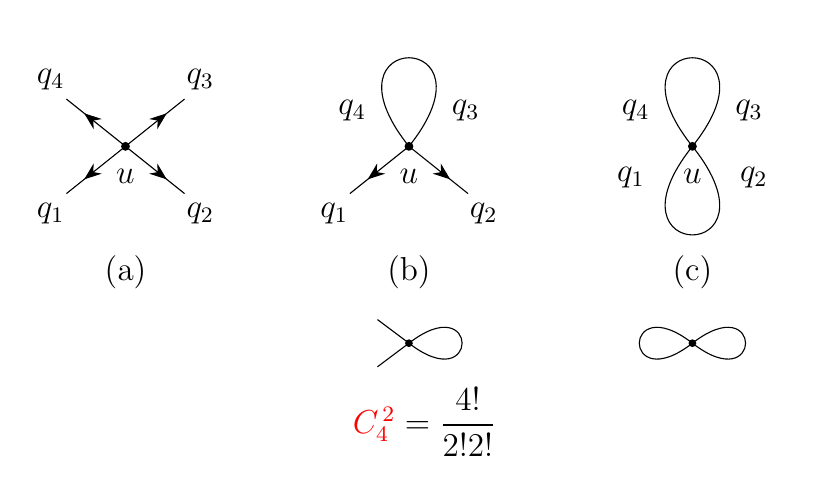
\begin{tikzpicture}[>=Stealth,scale=1.0,every node/.style={font=\large}]
  % (a)
  \begin{scope}[shift={(0,0)}]
    \fill (0,0) circle (1.6pt);
    \draw[meio=0.7] (0,0)--(-0.75,0.6);  \node at (-0.95,0.85) {$q_4$};
    \draw[meio=0.7] (0,0)--(0.75,0.6);   \node at (0.95,0.85) {$q_3$};
    \draw[meio=0.7] (0,0)--(-0.75,-0.6); \node at (-0.95,-0.85) {$q_1$};
    \draw[meio=0.7] (0,0)--(0.75,-0.6);  \node at (0.95,-0.85) {$q_2$};
    \node at (0,-0.38) {$u$};
    \node at (0,-1.6) {(a)};
  \end{scope}
  % (b)
  \begin{scope}[shift={(3.6,0)}]
    \fill (0,0) circle (1.6pt);
    \draw (0,0) .. controls (-1.2,1.5) and (1.2,1.5) .. (0,0);
    \node at (-0.72,0.45) {$q_4$}; \node at (0.72,0.45) {$q_3$};
    \draw[meio=0.7] (0,0)--(-0.75,-0.6); \node at (-0.95,-0.85) {$q_1$};
    \draw[meio=0.7] (0,0)--(0.75,-0.6);  \node at (0.95,-0.85) {$q_2$};
    \node at (0,-0.38) {$u$};
    \node at (0,-1.6) {(b)};
    \begin{scope}[shift={(0,-2.5)}]
      \fill (0,0) circle (1.4pt);
      \draw (0,0)--(-0.4,0.3); \draw (0,0)--(-0.4,-0.3);
      \draw (0,0) .. controls (0.9,0.7) and (0.9,-0.7) .. (0,0);
    \end{scope}
    \node at (0.2,-3.5) {$\corr{C_4^{\,2}}=\dfrac{4!}{2!2!}$};
  \end{scope}
  % (c)
  \begin{scope}[shift={(7.2,0)}]
    \fill (0,0) circle (1.6pt);
    \draw (0,0) .. controls (-1.2,1.5) and (1.2,1.5) .. (0,0);
    \draw (0,0) .. controls (-1.2,-1.5) and (1.2,-1.5) .. (0,0);
    \node at (-0.72,0.45) {$q_4$}; \node at (0.72,0.45) {$q_3$};
    \node at (-0.78,-0.4) {$q_1$}; \node at (0.78,-0.4) {$q_2$};
    \node at (0,-0.38) {$u$};
    \node at (0,-1.6) {(c)};
    \begin{scope}[shift={(0,-2.5)}]
      \fill (0,0) circle (1.4pt);
      \draw (0,0) .. controls (0.9,0.7) and (0.9,-0.7) .. (0,0);
      \draw (0,0) .. controls (-0.9,0.7) and (-0.9,-0.7) .. (0,0);
    \end{scope}
  \end{scope}
\end{tikzpicture}
\caption{Grafos de primeira ordem em $u$.}
\end{figure}
\noindent\nota{c:fig2}{notação: na figura original está escrito ``$C_2^{\,4}=4!/2!2!$'';
o texto, eq.~(99), usa $C_4^{\,2}$. Figura redesenhada.}


Temos então a contribuição (para o termo de dois spins),
\begin{equation}
-6\frac{u}{4!}\frac{1}{N^d}\sum_{|q_1|<1/b}\ \sum_{|q_2|<1/b}\left[\sum_{|q_3|>1/b}\frac{1}{r+q_3^2}\right]\sh_{q_1}\sh_{q_2}\delta_{q_1+q_2,0}.
\end{equation}
Introduzindo a definição
\begin{equation}
A=\frac{1}{N^d}\sum_{|q_3|>1/b}\frac{1}{r+q_3^2}=\frac{1}{\left(2\pi\right)^d}\int_{|q_3|>1/b}d^dq_3\,\frac{1}{r+q_3^2},
\end{equation}
em que $A$ depende apenas de $r$ \corr{(e de $b$)} (isto é, em que $A$ é uma constante em
\corr{ordem dominante} em $r$), a contribuição perturbativa desse termo é dada por
\nota{c:Aconst}{no original, ``$A$ é uma constante em primeira ordem em $r$''. Uma constante é o termo de
ordem \emph{zero} em $r$: $A=A_0-B_0r+O(r^2)$, com $A_0=A(r=0)$; o termo linear é o que aparece em (133).
Em (102), e em (122), (130), (131), ``$|q|>1/b$'' significa a coroa $1/b<|q|<1$.}
\begin{equation}
-6\frac{u}{4!}A\sum_{|q_1|<1/b}\ \sum_{|q_2|<1/b}\sh_{q_1}\sh_{q_2}\delta_{q_1+q_2,0}.
\end{equation}

Introduzindo finalmente os \corr{reescalonamentos} de praxe, temos a contribuição
para o termo de dois spins,
\nota{c:resc}{digitação: no original, ``rescalonamentos''.}
\begin{equation}
-6\frac{u}{4!}A\frac{\left(N'\right)^d}{\left(2\pi\right)^d}\int_{q'<1}d^dq'\,b^2\sh'_{q'}\sh'_{-q'}.
\end{equation}

(iii) finalmente, há uma última possibilidade, com os quatro vetores de
onda na coroa externa. Essa contribuição, que está associada ao grafo da
figura 2 (c), fornece apenas uma constante trivial.

Para simplificar, vamos escrever o hamiltoniano transformado a campo
nulo ($H=0$),
\begin{equation}
\begin{split}
\Hb'=\corr{-}\frac12&\frac{\left(N'\right)^d}{\left(2\pi\right)^d}\int_0^1d^dq'\left[b^2r\cmais q'^2+O\left(q'^4\right)\right]\sh'_{q'}\sh'_{-q'}
-6\frac{u}{4!}A\frac{\left(N'\right)^d}{\left(2\pi\right)^d}\int_0^1d^dq'\,b^2\sh'_{q'}\sh'_{-q'}-\\
&-b^{4-d}\frac{u}{4!}\frac{1}{\left(N'\right)^d}\frac{\left(N'\right)^{3d}}{\left(2\pi\right)^{3d}}\int d^dq'_1d^dq'_2d^dq'_3\,\sh'_{q_1}\sh'_{q_2}\sh'_{q_3}\sh\corr{'}_{-q_1-q_2-q_3}.
\end{split}
\end{equation}
\ver{c:rconv}
\nota{c:prime105}{notação: no original falta a plica no último spin,
``$\sh_{-q_1-q_2-q_3}$'' (o mesmo em (125)); todos são variáveis reescalonadas, e os índices
$q_i$ devem ser lidos como $q'_i$. No PDF original a primeira linha desta equação ultrapassa a margem.}

Então temos as relações de recorrência,
\begin{equation}
r'=b^2r+\frac12Ab^2u
\end{equation}
e
\begin{equation}
u'=b^{4-d}u.
\end{equation}
\nota{c:rec106}{conferência do sinal de (106): em (105), juntando os dois termos quadráticos,
$-\tfrac12\left[b^2r+q'^2\right]-\tfrac{6}{4!}Ab^2u=-\tfrac12\left[b^2\left(r+\tfrac12Au\right)+q'^2\right]$,
que comparado com $-\tfrac12[r'+q'^2]$ dá $r'=b^2r+\tfrac12Ab^2u$. O sinal $+$ está correto
\emph{com a definição corrigida de $r$}; com a definição original, $[\,r-q^2\,]$, a mesma conta daria
$r'=b^2r-\tfrac12Ab^2u$ (C\ref{c:rconv}).}

De novo, surge apenas o ponto fixo trivial,
\begin{equation}
r^*=u^*=0,
\end{equation}
característico do modelo \corr{gaussiano}, com os autovalores
\nota{c:gauss}{digitação: no original, ``gausssiano''.}
\begin{equation}
\Lambda_1=b^2\to\lambda_1=2,
\end{equation}
que é associado a um operador relevante (operador energia), que define o
comportamento crítico de natureza térmica (como no modelo gaussiano), e
\begin{equation}
\Lambda_2=b^{4-d}\to\lambda_2=4-d,
\end{equation}
associado a um operador irrelevante quando $d>4$.

Esses autovalores indicam uma situação peculiar: o ponto fixo trivial se
torna fisicamente inaceitável para $d<4$ (nos casos de interesse real). O
que será que acontece para $d<4$? Esse resultado nos obriga a ir adiante,
a fazer uma tentativa de realizar um cálculo até uma ordem superior, a fim
de analisar o que acontece para $d<4$ (incluindo o caso de interesse físico,
$d=3$).

% ------------------------------------------------------------
\subsection{Cálculo de segunda ordem em $\epsilon=4-d$}
% ------------------------------------------------------------

Em segunda ordem, as relações de recorrência podem conter termos
proporcionais a $u^2$. Antes de qualquer cálculo, vamos estudar o efeito de um termo
de segunda ordem na relação de recorrência para o parâmetro associado ao
operador de quatro spins. Vamos supor que
\begin{equation}
r'=b^2r+\frac12Ab^2u
\end{equation}
e que
\begin{equation}
u'=b^{4-d}u-\frac32Bb^{4-d}u^2,
\end{equation}
em que o termo extra, escrito de forma conveniente, depende de uma
determinada constante $B$. Esse sistema admite duas soluções:

(i) o ponto fixo trivial,
\begin{equation}
r^*=u^*=0,
\end{equation}
de natureza gaussiana, que não é fisicamente aceitável para $d<4$;

\corr{(ii)} novo ponto fixo, dado por
\nota{c:ii}{digitação: no original os dois itens estão numerados ``(i)''.}
\begin{equation}
u^*=\frac{b^{\epsilon}-1}{\frac32Bb^{\epsilon}}\to\frac{2\ln b}{3B_0}\epsilon,
\end{equation}
para $\epsilon=4-d\to0$, e
\begin{equation}
r^*=-\frac{A_0b^2\ln b}{3B_0\left(b^2-1\right)}\epsilon,
\end{equation}
em que $r^*$ e $u^*$ são de ordem $\epsilon$, de acordo com o ``\corr{Ansatz}'' de Wilson e
Fisher.
\nota{c:ansatz}{grafia: no original, ``Anzatz''.}
Embora $A$ e $B$ possam depender de $r$, deve ser suficiente, até ordem
$\epsilon$, considerar os valores constantes $A_0$ e $B_0$ (ou seja, valores assumidos por
$A$ e $B$ quando $r^*=0$). Até a ordem dos nossos cálculos, também não
há contribuição de um eventual termo adicional, de ordem $u^2$, na primeira
relação de recorrência, para o parâmetro $r'$.

Vamos então verificar se esse tipo de estrutura pode ser realmente obtido
a partir dos nossos cálculos.

Em segunda ordem, a contribuição para o termo quártico deve ser
proveniente de termos do tipo
\begin{multline}
\frac12\left(-\frac{u}{4!}\right)\frac{1}{N^d}\sum_{|q_1|<1/b}\ \sum_{|q_{\corr{2}}|>1/b}\ \sum_{|q_3|>1/b}\ \sum_{|q_4|<1/b}\sh_{q_1}\sh_{q_2}\sh_{q_3}\sh_{q_4}\delta_{q_1+q_2+q_3+q_4,0}\times\\
\times\left(-\frac{u}{4!}\right)\frac{1}{N^d}\sum_{|q_5|>1/b}\ \sum_{|q_6|<1/b}\ \sum_{|q_7|<1/b}\ \sum_{|q_8|>1/b}\sh_{q_5}\sh_{q_6}\sh_{q_7}\sh_{q_8}\delta_{\corr{q_5+q_6+q_7+q_8,0}},
\end{multline}
\nota{c:delta116}{notação: no original o segundo delta aparece sem índices (``$\delta,$'') e o
limite da segunda soma está escrito ``$|q2|$'', aqui e em (118).}
em que estamos usando a notação da figura 3.

\begin{figure}[H]
\centering
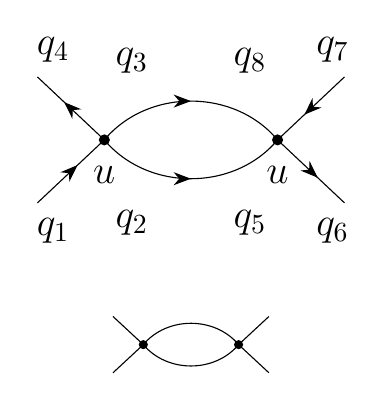
\begin{tikzpicture}[>=Stealth,every node/.style={font=\Large}]
  \fill (-1.1,0) circle (2pt); \fill (1.1,0) circle (2pt);
  \draw[meio=0.5] (-1.1,0) to[bend left=50] (1.1,0);
  \draw[meio=0.5] (-1.1,0) to[bend right=50] (1.1,0);
  \draw[meio=0.6] (-1.1,0)--(-1.95,0.8);  \node at (-1.75,1.15) {$q_4$};
  \draw[meio=0.6] (-1.95,-0.8)--(-1.1,0); \node at (-1.75,-1.15) {$q_1$};
  \draw[meio=0.6] (1.95,0.8)--(1.1,0);    \node at (1.8,1.15) {$q_7$};
  \draw[meio=0.6] (1.1,0)--(1.95,-0.8);   \node at (1.8,-1.15) {$q_6$};
  \node at (-0.75,1.0) {$q_3$}; \node at (0.75,1.0) {$q_8$};
  \node at (-0.75,-1.05) {$q_2$}; \node at (0.75,-1.05) {$q_5$};
  \node at (-1.1,-0.45) {$u$}; \node at (1.1,-0.45) {$u$};
  \begin{scope}[shift={(0,-2.6)},scale=0.55]
    \fill (-1.1,0) circle (3pt); \fill (1.1,0) circle (3pt);
    \draw (-1.1,0) to[bend left=50] (1.1,0);
    \draw (-1.1,0) to[bend right=50] (1.1,0);
    \draw (-1.1,0)--(-1.8,0.65); \draw (-1.1,0)--(-1.8,-0.65);
    \draw (1.1,0)--(1.8,0.65);  \draw (1.1,0)--(1.8,-0.65);
  \end{scope}
\end{tikzpicture}
\caption{Grafo de segunda ordem que contribui para o termo de quatro spins.}
\end{figure}
\noindent{\color{red}\small[figura redesenhada]}


Devido à estrutura dos
cumulantes, não há contribuição de termos associados a grafos desconexos (que
se cancelam) e há um fator $1/2$ inicial. Além disso, precisamos levar em
conta a multiplicidade desses termos, que é proveniente das escolhas das
``contrações'' gaussianas. Não é difícil perceber que precisamos escolher duas
patas de cada vértice, e que ainda há um fator 2, pois a primeira pata
escolhida pode ser ligada a cada uma das duas escolhas do outro vértice. Assim
temos a multiplicidade (ver figura 3)
\begin{equation}
C_4^2\times C_4^2\times2=\frac18\left(4!\right)^2.
\end{equation}
Em resumo, temos a contribuição
\begin{multline}
\frac{u^2}{16}\frac{1}{N^{2d}}\sum_{|q_1|<1/b}\ \sum_{|q_{\corr{2}}|>1/b}\ \sum_{|q_3|>1/b}\ \sum_{|q_4|<1/b}\ \corr{\sum_{|q_5|>1/b}}\ \sum_{|q_6|<1/b}\ \sum_{|q_7|<1/b}\ \corr{\sum_{|q_8|>1/b}}
\sh_{q_1}\sh_{q_4}\sh_{q_6}\sh_{q_7}\times\\
\times\left\langle\sh_{q_2}\sh_{q_5}\right\rangle_{0>}\left\langle\sh_{q_3}\sh_{q_8}\right\rangle_{0>}\delta_{q_1+q_2+q_3+q_4,0}\,\delta_{q_5+q_6+q_7+q_8,0}\,.
\end{multline}
\nota{c:sum118}{notação: no original faltam as somas sobre $q_5$ e $q_8$, que também são somados
[e depois eliminados pelos deltas de (119) e (120)]. O prefator está certo:
$\tfrac12\cdot\tfrac{1}{(4!)^2}\cdot\tfrac{(4!)^2}{8}=\tfrac1{16}$.}

Levando em conta a expressão das correlações gaussianas,
\begin{equation}
\left\langle\sh_{q_2}\sh_{q_5}\right\rangle_{0>}=\frac{1}{r+q_2^2}\delta_{q_2+q_5,0}
\end{equation}
e
\begin{equation}
\left\langle\sh_{q_3}\sh_{q_8}\right\rangle_{0>}=\frac{1}{r+q_3^2}\delta_{q_3+q_8,0},
\end{equation}
temos
\begin{multline}
\frac{u^2}{16}\frac{1}{N^{2d}}\sum_{|q_1|<1/b}\ \sum_{|q_4|<1/b}\ \sum_{|q_6|<1/b}\ \sum_{|q_7|<1/b}\sh_{q_1}\sh_{q_4}\sh_{q_6}\sh_{q_7}\delta_{q_1+q_4+q_6+q_7,0}\times\\
\times\left(\sum_{|q_2|>1/b}\frac{1}{r+q_2^2}\right)\left(\sum_{|q_3|>1/b}\frac{1}{r+q_3^2}\right)\delta_{q_2+q_3,q_6+q_7}.
\end{multline}
Torna-se agora conveniente definir
\begin{equation}
\begin{split}
B&=\frac{1}{N^d}\left(\sum_{|q_2|>1/b}\frac{1}{r+q_2^2}\right)\left(\sum_{|q_3|>1/b}\frac{1}{r+q_3^2}\right)\delta_{q_2+q_3,q_6+q_7}=\\
&=\frac{1}{N^d}\sum_{|q_2|>1/b}\frac{1}{r+q_2^2}\,\frac{1}{r+\left(-q_2+q_6+q_7\right)^2}=\\
&=\frac{1}{\corr{\left(2\pi\right)^d}}\int_{|q|>1/b}d^dq\,\frac{1}{r+q^2}\,\frac{1}{r+\left(-q+q_6+q_7\right)^2}=\\
&=\frac{1}{\corr{\left(2\pi\right)^d}}\int_{|q|>1/b}d^dq\,\frac{1}{\left(r+q^2\right)^2}+O\left(q_6,q_7\right).
\end{split}
\end{equation}
\nota{c:2pi122}{digitação: no original, ``$(2\pi^d)$'' nas duas últimas linhas (e na eq.~(131));
o correto é $(2\pi)^d$, como em (102) e (130).}

Pode-se mostrar que os termos dependentes dos momentos $q_6$ e $q_7$ estão
associados a operadores irrelevantes (como foi calculado explicitamente no
caso dos termos de ordem $q^4$ para o modelo gaussiano). Portanto, vamos
descartar termos dessa natureza, bem como contribuições perturbativas de
seis ou mais spins, que também são irrelevantes (note que em segunda ordem
apareceria uma contribuição para o termo de seis spins). Uma análise muito
simples, de caráter dimensional, seria suficiente para discutir essas questões,
apenas aparentemente mais sutis (o leitor interessado deve consultar o artigo
de revisão de Wilson e Kogut, citado nas referências).

Temos então a contribuição para o termo quártico,
\begin{equation}
\frac{u^2}{16}\frac{1}{N^d}B\sum_{|q_1|<1/b}\ \sum_{|q_4|<1/b}\ \sum_{|q_6|<1/b}\ \sum_{|q_7|<1/b}\sh_{q_1}\sh_{q_4}\sh_{q_6}\sh_{q_7}\delta_{q_1+q_4+q_6+q_7,0},
\end{equation}
com $B$ dado pela equação (122) sem os termos de ordem superior nos
momentos. Introduzindo os devidos reescalonamentos, e redefinindo de forma
conveniente as variáveis de momento, podemos escrever
\begin{equation}
\frac{u^2}{16}Bb^{4-d}\frac{1}{\left(N'\right)^d}\sum_{|q_1|<1}...\sum_{|q_4|<1}\sh'_{q_1}\sh'_{q_2}\sh'_{q_3}\sh'_{q_4}\delta_{q_1+q_2+q_3+q_4,0}.
\end{equation}
Adicionando este termo ao hamiltoniano transformado da equação (105),
temos
\begin{equation}
\begin{split}
\Hb'=\corr{-}\frac12&\frac{\left(N'\right)^d}{\left(2\pi\right)^d}\int_0^1d^dq'\left[b^2r\cmais q'^2+O\left(q'^4\right)\right]\sh'_{q'}\sh'_{-q'}
-6\frac{u}{4!}A\frac{\left(N'\right)^d}{\left(2\pi\right)^d}\int_0^1d^dq'\,b^2\sh'_{q'}\sh'_{-q'}\\
&-b^{4-d}\frac{u}{4!}\frac{1}{\left(N'\right)^d}\frac{\left(N'\right)^{3d}}{\left(2\pi\right)^{3d}}\int d^dq'_1d^dq'_2d^dq'_3\,\sh'_{q_1}\sh'_{q_2}\sh'_{q_3}\sh\corr{'}_{-q_1-q_2-q_3}+\\
&\cmais b^{4-d}\frac{u^2}{16}\corr{B}\frac{1}{\left(N'\right)^d}\frac{\left(N'\right)^{3d}}{\left(2\pi\right)^{3d}}\int d^dq'_1d^dq'_2d^dq'_3\,\sh'_{q_1}\sh'_{q_2}\sh'_{q_3}\sh\corr{'}_{-q_1-q_2-q_3}.
\end{split}
\end{equation}
\ver{c:rconv}
\nota{c:e125}{erro: no original a última linha é
``$+\,-b^{4-d}\frac{u^2}{16}\frac{1}{(N')^d}\cdots$'': o sinal está trocado e falta o fator $B$.
O termo de segunda ordem (124) é positivo e contém $B$. Só assim os dois termos quárticos somam
$-\frac{b^{4-d}}{4!}\left[u-\frac{4!}{16}Bu^2\right]=-\frac{b^{4-d}}{4!}\left[u-\frac32Bu^2\right]$,
que é a recorrência (127).}

Comparando com o hamiltoniano original a campo nulo, dado pela equação
(91), temos finalmente as relações de recorrência,
\begin{equation}
r'=b^2r+\frac12Ab^2u
\end{equation}
e
\begin{equation}
u'=b^{4-d}u-\frac32Bb^{4-d}u^2,
\end{equation}
exatamente na mesma forma como tinham sido escritas no início dessa seção
(ver equações 111 e 112). Como já foi visto, há um ponto fixo trivial, de
caráter gaussiano, $r^*=u^*=0$, que é instável para $d<4$. Vamos então
analisar o ponto fixo não trivial.

% ------------------------------------------------------------
\subsection{Análise de estabilidade do ponto fixo não trivial}
% ------------------------------------------------------------

No limite $\epsilon=4-d\to0$, o ponto fixo não trivial é dado pelas equações (114)
e (115),
\begin{equation}
u^*=\frac{b^{\epsilon}-1}{\frac32Bb^{\epsilon}}\to\frac{2\ln b}{3B_0}\epsilon
\end{equation}
e
\begin{equation}
r^*=-\frac{A_0b^2\ln b}{3B_0\left(b^2-1\right)}\epsilon.
\end{equation}
em que $A_0$ e $B_0$ são os valores de $A$ e $B$ para $r^*=0$.

A análise linear de estabilidade nas vizinhanças desse ponto fixo não
trivial requer certos cuidados. Vamos então recordar as definições
\begin{equation}
A=\frac{1}{\left(2\pi\right)^d}\int_{|q|>1/b}d^dq\,\frac{1}{r+q^2}
\end{equation}
e
\begin{equation}
B=\frac{1}{\corr{\left(2\pi\right)^d}}\int_{|q|>1/b}d^dq\,\frac{1}{\left(r+q^2\right)^2},
\end{equation}
\ver{c:2pi122}
em que estamos considerando a expressão de $B$ para momentos internos
nulos. A partir das relações de recorrência, temos
\begin{equation}
\left(\frac{\partial r'}{\partial r}\right)_*=b^2+\frac12\left(\frac{\partial A}{\partial r}\right)_*b^2u^{\corr{*}}+O\left(\epsilon^2\right),
\end{equation}
em que
\begin{equation}
\left(\frac{\partial A}{\partial r}\right)=-\frac{1}{\left(2\pi\right)^d}\int_{|q|>1/b}d^dq\,\frac{1}{\left(r+q^2\right)^2}=-B.
\end{equation}
Portanto,
\begin{equation}
\left(\frac{\partial r'}{\partial r}\right)_*=b^2-\frac12B_0b^2u^{\corr{*}}+O\left(\epsilon^2\right)=b^2-\frac{b^2\ln b}{3}\epsilon+O\left(\epsilon^2\right).
\end{equation}
\nota{c:ustar}{notação: no original, ``$u_*$'' em (132) e (134); é o mesmo $u^*$ de (128).}
As outras derivadas necessárias para a análise linear de estabilidade são dadas
por
\begin{equation}
\left(\frac{\partial r'}{\partial u}\right)_*=\frac12A_0b^2+O\left(\epsilon\right),
\end{equation}
\begin{equation}
\left(\frac{\partial u'}{\partial r}\right)_*=O\left(\epsilon^2\right)
\end{equation}
e
\begin{equation}
\left(\frac{\partial u'}{\partial u}\right)_*=b^{4-d}-3B_0b^{4-d}u^*+O\left(\epsilon^2\right)=1-\epsilon\ln b+O\left(\epsilon^2\right),
\end{equation}
em que ocorreram alguns cancelamentos absolutamente notáveis!

Temos assim a forma linear
\begin{equation}
\left(\begin{array}{c}\Delta r'\\ \Delta u'\end{array}\right)=
\left(\begin{array}{cc}b^2-\epsilon\frac13b^2\ln b+O\left(\epsilon^2\right)&\frac12A_0b^2+O\left(\epsilon\right)\\
O\left(\epsilon^2\right)&1-\epsilon\ln b+O\left(\epsilon^2\right)\end{array}\right)
\left(\begin{array}{c}\Delta r\\ \Delta u\end{array}\right),
\end{equation}
de onde vêm os autovalores
\begin{equation}
\Lambda_1=b^2-\epsilon\frac13b^2\ln b+O\left(\epsilon^2\right),
\end{equation}
que está associado a um operador relevante, e
\begin{equation}
\Lambda_2=1-\epsilon\ln b+O\left(\epsilon^2\right),
\end{equation}
que está associado a um operador irrelevante para $\epsilon>\corr{0}$ (isto é, na situação
de interesse físico, $d<4$).
\nota{c:eps0}{erro: no original, ``para $\epsilon>1$''. $\Lambda_2<1$ para qualquer $\epsilon>0$, isto é,
$d<4$; $\epsilon>1$ corresponderia a $d<3$.}
Na figura 4, para $d<4$, representamos os fluxos
das relações de recorrência no espaço $r-u$ de parâmetros (o ponto fixo não
trivial, do ``tipo Ising'', tem caráter hiperbólico; o ponto fixo gaussiano é
completamente instável).

Até primeira ordem em $\epsilon$, também podemos escrever
\begin{equation}
\lambda_1=\frac{\ln\Lambda_1}{\ln b}=2-\frac13\epsilon
\end{equation}
e
\begin{equation}
\lambda_2=\frac{\ln\Lambda_2}{\ln b}=-\epsilon.
\end{equation}
Os expoentes $\nu$, associado ao comprimento de correlação, e $\alpha$, associado ao
calor específico, são dados por
\[
\nu=\frac{1}{\lambda_1}=\frac12+\frac1{12}\epsilon+O\left(\epsilon^2\right)
\]
e
\begin{equation}
\alpha=2-\frac{d}{\lambda_1}=\frac16\epsilon+O\left(\epsilon^2\right).
\end{equation}
Para $\epsilon=0$ (isto é, $d=4$) recuperamos os valores de campo médio, $\nu=1/2$
e $\alpha=0$. Para $d=3$ ($\epsilon=1$) os valores são razoáveis. Em segunda ordem
em $\epsilon$, os valores obtidos podem ser favoravelmente comparados com os
melhores resultados das análises de expansões em série ou simulações numéricas.
No entanto, para levar adiante esse cálculo torna-se imprescindível utilizar
técnicas bem mais controladas de teoria de campos, que estão além dos
objetivos do nosso curso (ver o texto de Daniel Amit, citado nas referências). De
qualquer forma, na análise do comportamento crítico, o método de
Wilson-Fisher já faz parte da ``cultura'' da área, devendo ser utilizado em ``primeira
instância'' para complementar ou substituir com muitas vantagens os cálculos
usuais de campo médio.

\begin{figure}[H]
\centering
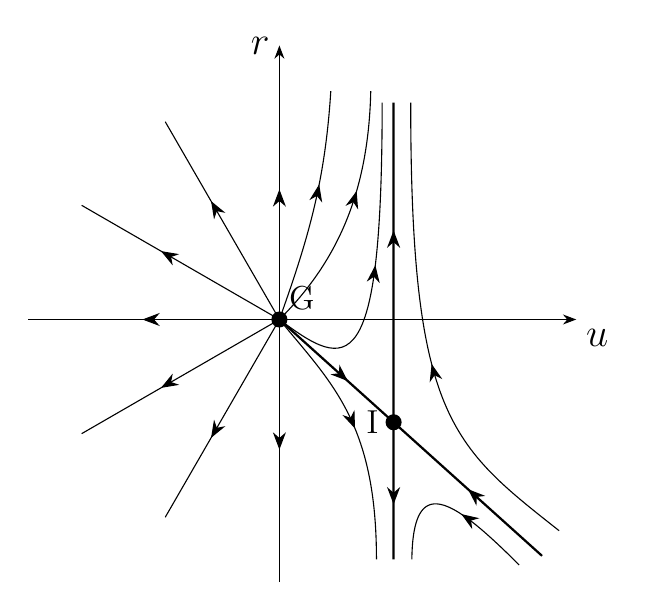
\begin{tikzpicture}[>=Stealth,scale=1.45]
  % eixos
  \draw[->] (-2.2,0)--(2.6,0) node[below right] {\Large $u$};
  \draw[->] (0,-2.3)--(0,2.4) node[left] {\Large $r$};
  % pontos fixos
  \coordinate (G) at (0,0);
  \coordinate (I) at (1.0,-0.9);
  % raios saindo de G (semiplano u<0 e eixo r)
  \foreach \a in {120,150,180,210,240}
    \draw[meio=0.6] (G)--(\a:2.0);
  \draw[meio=0.6] (G)--(0,1.9);
  \draw[meio=0.6] (G)--(0,-1.9);
  % curvas saindo de G com u>0
  \draw[meio=0.6] (G) .. controls (0.25,0.7) and (0.4,1.2) .. (0.45,2.0);
  \draw[meio=0.6] (G) .. controls (0.5,0.5) and (0.78,1.1) .. (0.8,2.0);
  \draw[meio=0.5] (G) .. controls (0.6,-0.45) and (0.9,-0.55) .. (0.9,1.9);
  \draw[meio=0.5] (G) .. controls (0.45,-0.55) and (0.85,-0.9) .. (0.85,-2.1);
  % linha critica (variedade estavel de I)
  \draw[thick,meio=0.6] (G)--(I);
  \draw[thick,meio=0.5] (2.3,-2.07)--(I);
  % variedade instavel de I
  \draw[thick,meio=0.6] (I)--(1.0,1.9);
  \draw[thick,meio=0.6] (I)--(1.0,-2.1);
  % curvas vindas de u grande
  \draw[meio=0.45] (2.45,-1.85) .. controls (1.5,-1.1) and (1.15,-0.85) .. (1.15,1.9);
  \draw[meio=0.45] (2.1,-2.15) .. controls (1.5,-1.55) and (1.17,-1.35) .. (1.16,-2.1);
  \fill (G) circle (2pt) node[above right] {\large G};
  \fill (I) circle (2pt) node[left=2pt] {\large I};
\end{tikzpicture}
\caption{Esboço das linhas de fluxo no espaço de parâmetros, \textcolor{red}{$r-u$}, para
$d<4$. Também estão indicados os pontos fixos: gaussiano (G), de caráter
instável, e Ising (I), de caráter hiperbólico.}
\end{figure}
\noindent\nota{c:fig4cap}{notação: no original, ``$r^*-u^*$''; o plano é o dos parâmetros $r$ e $u$
($r^*$, $u^*$ são as coordenadas dos pontos fixos). Figura redesenhada com a mesma topologia:
I em $u^*>0$, $r^*<0$; a linha G--I é a linha crítica, e a direção instável de I é a de $r$.}



\textbf{Referências:}

\textbf{1-} M. E. Fisher, ``The renormalization group in the theory of critical
behavior'', Rev. Mod. Phys. \textbf{46}, 597-616 (1974). Talvez este seja o trabalho
de revisão mais próximo do espírito do nosso curso. Ver também o ponto de
vista de Michael Fisher cerca de vinte anos depois: M. E. Fisher,
``Renormalization group theory: Its basis and formulation in statistical physics'', Rev.
Mod. Phys. \textbf{70}, 653-681 (1998). Ver ainda reminiscências mais recentes de
Michael Fisher: ``Renormalization group theory, the epsilon expansion and
Ken Wilson as I knew him'', Int. J. Mod. Phys. B \textbf{29}, 1530006 (2015).

\textbf{2-} K. G. Wilson e J. Kogut, ``The renormalization group and the $\epsilon$
expansion'', Phys. Rep. \textbf{12}, 75-200 (1974). Discussão detalhada de todas as
sutilezas da expansão de Wilson-Fisher.

\textbf{3-} J. J. Binney, N. J. Dowrick, A. J. Fisher e M. E. J. Newman, ``The
theory of critical phenomena: An introduction to the renormalization group'',
Oxford Science Publications, 1992. Texto didático, com ótima exposição
sobre as expansões diagramáticas (vai bem além do nosso curso).

\textbf{4-} D. J. Amit, ``Field theory, the renormalization group and critical
phenomena'', McGraw-Hill, 1978 (edição revista, World Scientific, 1993).
Exposição típica sobre a utilização de métodos de teoria de campos em
problemas de física estatística.

revisto em 2/11/2026

% ============================================================
% APENDICES DESTA REVISAO (tudo em vermelho)
% ============================================================
\newpage
{\color{red}
\section*{Apêndice A --- Lista das correções}

Tipos: \textbf{E} = erro de conta, de sinal ou de conceito; \textbf{N} = notação ou índices;
\textbf{D} = digitação ou grafia; \textbf{O} = observação (o original não está errado, mas
merece um esclarecimento). As páginas são as do PDF original.

\small
\begin{longtable}{@{}p{0.9cm}p{2.9cm}p{0.6cm}p{10.6cm}@{}}
\toprule
Nº & Local & Tipo & Correção\\
\midrule
\endhead
\bottomrule
\endfoot
\Cref{c:renorm} & p.~2, introdução & D & ``renormaliçao'' $\to$ renormalização; ``esse tipo hamiltoniano'' $\to$ esse tipo de hamiltoniano.\\
\Cref{c:strat} & p.~2, introdução & D & ``Stratonovitch'' $\to$ Stratonovich.\\
\Cref{c:qpi} & p.~5, eq.~(15) & O & O modo de borda $q=\pi$ também é real; sem efeito no limite termodinâmico.\\
\Cref{c:paren} & p.~6, após (20) & D & Parêntese a mais em ``$\Kh(q)=\Kh(-q))$''.\\
\Cref{c:scal} & p.~7, após (27) & O & No modelo gaussiano só $\gamma$ e $\Delta=\beta+\gamma$ ficam definidos; $\Delta=3/2$ apenas em $d=4$.\\
\Cref{c:d2} & p.~7, após (30) & E & ``diverge para $d<2$'' $\to$ $d\leq2$ (divergência logarítmica em $d=2$).\\
\Cref{c:c32} & p.~7, eq.~(32) & E & Falta o expoente 2: denominador $[\Delta T+\beta Jq^2]^2$.\\
\Cref{c:d4log} & p.~8, após (34) & E & ``não diverge para $d\geq4$'' $\to$ $d>4$; em $d=4$, $c\sim-\ln t$.\\
\Cref{c:sum35} & p.~8, eq.~(35) & N & Soma sobre $q$ $\to$ soma dupla sobre $q$ e $q'$.\\
\Cref{c:par42} & p.~9, eq.~(42) & D & Falta fechar o parêntese em $\exp[iq\cdot(r-r')]$.\\
\Cref{c:cm} & p.~9, após (43) & D & ``cm cuidado'' $\to$ com cuidado.\\
\Cref{c:dq47} & p.~9, eq.~(47) & N & ``$dr$'' $\to$ $dq$ no elemento de volume.\\
\Cref{c:ang47} & p.~9, após (47) & E & Limites angulares: $0$ a $\pi$ para $\theta_1,\dots,\theta_{d-2}$; $0$ a $2\pi$ só para $\theta_{d-1}$.\\
\Cref{c:polos} & p.~10, após (49) & D & ``pelo polos'' $\to$ pelos polos.\\
\Cref{c:oz53} & p.~10, eq.~(53) & O & Forma exata só em $d=3$; em geral vale (57) corrigida.\\
\Cref{c:i57} & p.~11, eq.~(57) & E & Falta o fator $1/r^{d-2}$: $I\sim r^{-(d-2)}(\kappa r)^{(d-3)/2}e^{-\kappa r}$.\\
\Cref{c:nu57} & p.~11, após (57) & E & ``$\nu=1$'' $\to$ $\nu=1/2$.\\
\Cref{c:lambda} & p.~12, seção 1.3 & E & ``grandes comprimentos de onda (curtas distâncias)'' $\to$ pequenos comprimentos de onda.\\
\Cref{c:h0} & p.~12, eq.~(61) & O & $\Hb_0\equiv\Hb_G$ (mudança de nome não anunciada).\\
\Cref{c:rconv} & p.~13, eq.~(65); também (66), (67), (70), (71), (89), (90), (91), (94), (105), (125) & E &
Sinal de $r$: a definição $r=(2\beta Jd-1)/\beta J$ é incompatível com o propagador $1/(r+q^2)$ e com as
recorrências usadas de (100) em diante. Corrigido para $r=(1-2\beta Jd)/\beta J$, com $-\frac12[r+q^2]$
no hamiltoniano.\\
\Cref{c:sefeitas} & p.~18, após (91) & D & ``devem se feitas'' $\to$ devem ser feitas.\\
\Cref{c:coroa} & p.~19, item (ii) & E & ``fora da coroa'' $\to$ fora do caroço.\\
\Cref{c:fig2} & p.~20, figura 2 & N & ``$C_2^{\,4}$'' $\to$ $C_4^{\,2}$, como na eq.~(99).\\
\Cref{c:Aconst} & p.~20, após (102) & E & ``constante em primeira ordem em $r$'' $\to$ em ordem dominante (ordem zero); $A$ depende também de $b$; a integral é sobre a coroa $1/b<|q|<1$.\\
\Cref{c:resc} & p.~20, antes de (104) & D & ``rescalonamentos'' $\to$ reescalonamentos.\\
\Cref{c:prime105} & p.~21, eq.~(105) & N & Falta a plica em $\sh'_{-q_1-q_2-q_3}$; linha além da margem.\\
\Cref{c:rec106} & p.~21, eq.~(106) & O & Conferência do sinal $+\frac12Ab^2u$ (correto com a definição corrigida de $r$).\\
\Cref{c:gauss} & p.~21, após (108) & D & ``gausssiano'' $\to$ gaussiano.\\
\Cref{c:ii} & p.~22, antes de (114) & D & Segundo item ``(i)'' $\to$ (ii).\\
\Cref{c:ansatz} & p.~22, após (115) & D & ``Anzatz'' $\to$ Ansatz.\\
\Cref{c:delta116} & p.~22--23, eq.~(116) & N & Delta sem índices $\to$ $\delta_{q_5+q_6+q_7+q_8,0}$; ``$|q2|$'' $\to$ $|q_2|$.\\
\Cref{c:sum118} & p.~23, eq.~(118) & N & Faltam as somas sobre $q_5$ e $q_8$.\\
\Cref{c:2pi122} & p.~24 e 26, eqs.~(122), (131) & D & ``$(2\pi^d)$'' $\to$ $(2\pi)^d$.\\
\Cref{c:e125} & p.~25, eq.~(125) & E & Última linha: sinal $-$ $\to$ $+$ e falta o fator $B$.\\
\Cref{c:ustar} & p.~26, eqs.~(132), (134) & N & ``$u_*$'' $\to$ $u^*$.\\
\Cref{c:eps0} & p.~27, após (140) & E & ``irrelevante para $\epsilon>1$'' $\to$ $\epsilon>0$.\\
\Cref{c:fig4cap} & p.~28, figura 4 & N & Legenda ``$r^*-u^*$'' $\to$ $r-u$.\\
\end{longtable}
\normalsize

\section*{Apêndice B --- Contas refeitas para conferir}

\textbf{1. Sinal de $r$ e o autovalor térmico} (C\ref{c:rconv}). Refazendo a análise linear
com as três combinações possíveis de sinais, até ordem $\epsilon$:

\begin{center}
\small\begin{tabular}{@{}p{6.4cm}ccc@{}}
\toprule
Combinação & $r^*$ & $\lambda_1$ & $\nu$\\
\midrule
$r'=b^2r+\frac12Ab^2u$, $A=\int(r+q^2)^{-1}$, $\partial A/\partial r=-B$\newline
(eqs.~(100)--(134) do original; coerente com $r=\Delta T/\beta J$) &
$-\dfrac{A_0b^2\ln b}{3B_0(b^2-1)}\epsilon$ & $2-\dfrac\epsilon3$ & $\dfrac12+\dfrac\epsilon{12}$\\[10pt]
$r'=b^2r-\frac12Ab^2u$, $A=\int(q^2-r)^{-1}$, $\partial A/\partial r=+B$\newline
(coerente com $r=(2\beta Jd-1)/\beta J$) &
$+\dfrac{A_0b^2\ln b}{3B_0(b^2-1)}\epsilon$ & $2-\dfrac\epsilon3$ & $\dfrac12+\dfrac\epsilon{12}$\\[10pt]
$r'=b^2r-\frac12Ab^2u$, $A=\int(r+q^2)^{-1}$, $\partial A/\partial r=-B$\newline
(trocar só o sinal da recorrência) &
$+\dfrac{A_0b^2\ln b}{3B_0(b^2-1)}\epsilon$ & $2+\dfrac\epsilon3$ & $\dfrac12-\dfrac\epsilon{12}$ (errado)\\
\bottomrule
\end{tabular}
\end{center}

As duas primeiras linhas são a mesma física escrita com $r\to-r$. A terceira é inconsistente.

\textbf{2. Valores explícitos de $A_0$ e $B_0$.} Com a zona esférica de raio 1 e $r=0$, e com
$K_d=2\pi^{d/2}/[\Gamma(d/2)(2\pi)^d]$,
\[
A_0=K_d\int_{1/b}^1q^{d-3}dq=K_d\,\frac{1-b^{2-d}}{d-2},\qquad
B_0=K_d\int_{1/b}^1q^{d-5}dq=K_d\,\frac{b^{\epsilon}-1}{\epsilon}\ \xrightarrow{\ \epsilon\to0\ }\ K_4\ln b ,
\]
com $K_4=1/8\pi^2$ e $A_0\to K_4(1-b^{-2})/2$ em $d=4$. Substituindo em (128) e (129),
\[
u^*=\frac{2\epsilon}{3K_4}=\frac{16\pi^2}{3}\epsilon,\qquad r^*=-\frac{\epsilon}{6},
\]
independentes de $b$, como deve ser, e iguais aos valores usuais da literatura.

\textbf{3. Eq.~(57)} (C\ref{c:i57}). A integral (56) foi calculada numericamente para $d=3,4,5$ e
$\kappa r=10,40,160$, e coincide com $2\pi^{d/2}(2\kappa/r)^{\frac d2-1}K_{\frac d2-1}(\kappa r)$.
A razão entre $I$ e a forma corrigida tende a uma constante ($19{,}74=2\pi^2$ em $d=3$; $49{,}6$ em
$d=4$; $124{,}8$ em $d=5$, para $\kappa r=160$), enquanto a razão entre $I$ e a forma original decresce como
$r^{-(d-2)}$.

\textbf{4. Calor específico em $d=4$} (C\ref{c:d4log}). $\int_0^1q^3dq/(t+q^2)^2=1{,}81;\ 4{,}11;\ 6{,}41$
para $t=10^{-2},10^{-4},10^{-6}$, isto é, $-\frac12\ln t-\frac12$.

\textbf{5. Multiplicidades e expoentes.} $C_4^2\times C_4^2\times2=72=(4!)^2/8$;
$\frac12\cdot72/(4!)^2=\frac1{16}$; $4!/16=\frac32$.
$1/(2-\epsilon/3)=\frac12+\frac{\epsilon}{12}+O(\epsilon^2)$ e
$2-(4-\epsilon)/(2-\epsilon/3)=\frac{\epsilon}{6}+O(\epsilon^2)$.

\textbf{6. Demais equações.} Foram refeitas, sem encontrar erro, as contas das eqs.~(7)--(10),
(17)--(20), (24)--(31), (36)--(52), (54)--(56), (64)--(77) [com o sinal de $r$ corrigido],
(81), (87), (96)--(104), (114)--(124) e (128)--(143).
}

\end{document}
